\documentclass[twoside]{book}

% Packages required by doxygen
\usepackage{fixltx2e}
\usepackage{calc}
\usepackage{doxygen}
\usepackage[export]{adjustbox} % also loads graphicx
\usepackage{graphicx}
\usepackage[utf8]{inputenc}
\usepackage{makeidx}
\usepackage{multicol}
\usepackage{multirow}
\PassOptionsToPackage{warn}{textcomp}
\usepackage{textcomp}
\usepackage[nointegrals]{wasysym}
\usepackage[table]{xcolor}

% Font selection
\usepackage[T1]{fontenc}
\usepackage[scaled=.90]{helvet}
\usepackage{courier}
\usepackage{amssymb}
\usepackage{sectsty}
\renewcommand{\familydefault}{\sfdefault}
\allsectionsfont{%
  \fontseries{bc}\selectfont%
  \color{darkgray}%
}
\renewcommand{\DoxyLabelFont}{%
  \fontseries{bc}\selectfont%
  \color{darkgray}%
}
\newcommand{\+}{\discretionary{\mbox{\scriptsize$\hookleftarrow$}}{}{}}

% Page & text layout
\usepackage{geometry}
\geometry{%
  a4paper,%
  top=2.5cm,%
  bottom=2.5cm,%
  left=2.5cm,%
  right=2.5cm%
}
\tolerance=750
\hfuzz=15pt
\hbadness=750
\setlength{\emergencystretch}{15pt}
\setlength{\parindent}{0cm}
\setlength{\parskip}{3ex plus 2ex minus 2ex}
\makeatletter
\renewcommand{\paragraph}{%
  \@startsection{paragraph}{4}{0ex}{-1.0ex}{1.0ex}{%
    \normalfont\normalsize\bfseries\SS@parafont%
  }%
}
\renewcommand{\subparagraph}{%
  \@startsection{subparagraph}{5}{0ex}{-1.0ex}{1.0ex}{%
    \normalfont\normalsize\bfseries\SS@subparafont%
  }%
}
\makeatother

% Headers & footers
\usepackage{fancyhdr}
\pagestyle{fancyplain}
\fancyhead[LE]{\fancyplain{}{\bfseries\thepage}}
\fancyhead[CE]{\fancyplain{}{}}
\fancyhead[RE]{\fancyplain{}{\bfseries\leftmark}}
\fancyhead[LO]{\fancyplain{}{\bfseries\rightmark}}
\fancyhead[CO]{\fancyplain{}{}}
\fancyhead[RO]{\fancyplain{}{\bfseries\thepage}}
\fancyfoot[LE]{\fancyplain{}{}}
\fancyfoot[CE]{\fancyplain{}{}}
\fancyfoot[RE]{\fancyplain{}{\bfseries\scriptsize Generated by Doxygen }}
\fancyfoot[LO]{\fancyplain{}{\bfseries\scriptsize Generated by Doxygen }}
\fancyfoot[CO]{\fancyplain{}{}}
\fancyfoot[RO]{\fancyplain{}{}}
\renewcommand{\footrulewidth}{0.4pt}
\renewcommand{\chaptermark}[1]{%
  \markboth{#1}{}%
}
\renewcommand{\sectionmark}[1]{%
  \markright{\thesection\ #1}%
}

% Indices & bibliography
\usepackage{natbib}
\usepackage[titles]{tocloft}
\setcounter{tocdepth}{3}
\setcounter{secnumdepth}{5}
\makeindex

% Hyperlinks (required, but should be loaded last)
\usepackage{ifpdf}
\ifpdf
  \usepackage[pdftex,pagebackref=true]{hyperref}
\else
  \usepackage[ps2pdf,pagebackref=true]{hyperref}
\fi
\hypersetup{%
  colorlinks=true,%
  linkcolor=blue,%
  citecolor=blue,%
  unicode%
}

% Custom commands
\newcommand{\clearemptydoublepage}{%
  \newpage{\pagestyle{empty}\cleardoublepage}%
}

\usepackage{caption}
\captionsetup{labelsep=space,justification=centering,font={bf},singlelinecheck=off,skip=4pt,position=top}

%===== C O N T E N T S =====

\begin{document}

% Titlepage & ToC
\hypersetup{pageanchor=false,
             bookmarksnumbered=true,
             pdfencoding=unicode
            }
\pagenumbering{alph}
\begin{titlepage}
\vspace*{7cm}
\begin{center}%
{\Large My Project }\\
\vspace*{1cm}
{\large Generated by Doxygen 1.8.13}\\
\end{center}
\end{titlepage}
\clearemptydoublepage
\pagenumbering{roman}
\tableofcontents
\clearemptydoublepage
\pagenumbering{arabic}
\hypersetup{pageanchor=true}

%--- Begin generated contents ---
\chapter{Hierarchical Index}
\section{Class Hierarchy}
This inheritance list is sorted roughly, but not completely, alphabetically\+:\begin{DoxyCompactList}
\item \contentsline{section}{main}{\pageref{classmain}}{}
\item Q\+Dialog\begin{DoxyCompactList}
\item \contentsline{section}{quests}{\pageref{classquests}}{}
\end{DoxyCompactList}
\item Q\+Graphics\+Pixmap\+Item\begin{DoxyCompactList}
\item \contentsline{section}{butb}{\pageref{classbutb}}{}
\item \contentsline{section}{butblack}{\pageref{classbutblack}}{}
\item \contentsline{section}{butg}{\pageref{classbutg}}{}
\item \contentsline{section}{butp}{\pageref{classbutp}}{}
\end{DoxyCompactList}
\item Q\+Graphics\+Scene\begin{DoxyCompactList}
\item \contentsline{section}{g2\+\_\+setup}{\pageref{classg2__setup}}{}
\end{DoxyCompactList}
\item Q\+Object\begin{DoxyCompactList}
\item \contentsline{section}{butb}{\pageref{classbutb}}{}
\item \contentsline{section}{butblack}{\pageref{classbutblack}}{}
\item \contentsline{section}{butg}{\pageref{classbutg}}{}
\item \contentsline{section}{butp}{\pageref{classbutp}}{}
\item \contentsline{section}{Centering}{\pageref{classCentering}}{}
\item \contentsline{section}{jsonhandler}{\pageref{classjsonhandler}}{}
\item \contentsline{section}{signup\+\_\+scene}{\pageref{classsignup__scene}}{}
\end{DoxyCompactList}
\item Q\+Widget\begin{DoxyCompactList}
\item \contentsline{section}{account}{\pageref{classaccount}}{}
\item \contentsline{section}{account\+\_\+dashboard}{\pageref{classaccount__dashboard}}{}
\item \contentsline{section}{account\+\_\+sidebar}{\pageref{classaccount__sidebar}}{}
\item \contentsline{section}{g1\+\_\+info}{\pageref{classg1__info}}{}
\item \contentsline{section}{g1\+\_\+settings}{\pageref{classg1__settings}}{}
\item \contentsline{section}{g1\+\_\+setup}{\pageref{classg1__setup}}{}
\item \contentsline{section}{g1\+\_\+startmenu}{\pageref{classg1__startmenu}}{}
\item \contentsline{section}{g2\+\_\+settings}{\pageref{classg2__settings}}{}
\item \contentsline{section}{g2\+\_\+startmenu}{\pageref{classg2__startmenu}}{}
\item \contentsline{section}{game\+Lost}{\pageref{classgameLost}}{}
\item \contentsline{section}{game\+Won}{\pageref{classgameWon}}{}
\item \contentsline{section}{no\+Turns}{\pageref{classnoTurns}}{}
\item \contentsline{section}{playasguest}{\pageref{classplayasguest}}{}
\item \contentsline{section}{scene1}{\pageref{classscene1}}{}
\item \contentsline{section}{signin\+Page}{\pageref{classsigninPage}}{}
\item \contentsline{section}{signup\+Page}{\pageref{classsignupPage}}{}
\item \contentsline{section}{time\+Up}{\pageref{classtimeUp}}{}
\end{DoxyCompactList}
\end{DoxyCompactList}

\chapter{Class Index}
\section{Class List}
Here are the classes, structs, unions and interfaces with brief descriptions\+:\begin{DoxyCompactList}
\item\contentsline{section}{\hyperlink{classaccount}{account} }{\pageref{classaccount}}{}
\item\contentsline{section}{\hyperlink{classaccount__dashboard}{account\+\_\+dashboard} }{\pageref{classaccount__dashboard}}{}
\item\contentsline{section}{\hyperlink{classaccount__sidebar}{account\+\_\+sidebar} }{\pageref{classaccount__sidebar}}{}
\item\contentsline{section}{\hyperlink{classbutb}{butb} }{\pageref{classbutb}}{}
\item\contentsline{section}{\hyperlink{classbutblack}{butblack} }{\pageref{classbutblack}}{}
\item\contentsline{section}{\hyperlink{classbutg}{butg} }{\pageref{classbutg}}{}
\item\contentsline{section}{\hyperlink{classbutp}{butp} }{\pageref{classbutp}}{}
\item\contentsline{section}{\hyperlink{classCentering}{Centering} }{\pageref{classCentering}}{}
\item\contentsline{section}{\hyperlink{classg1__info}{g1\+\_\+info} }{\pageref{classg1__info}}{}
\item\contentsline{section}{\hyperlink{classg1__settings}{g1\+\_\+settings} }{\pageref{classg1__settings}}{}
\item\contentsline{section}{\hyperlink{classg1__setup}{g1\+\_\+setup} }{\pageref{classg1__setup}}{}
\item\contentsline{section}{\hyperlink{classg1__startmenu}{g1\+\_\+startmenu} }{\pageref{classg1__startmenu}}{}
\item\contentsline{section}{\hyperlink{classg2__settings}{g2\+\_\+settings} }{\pageref{classg2__settings}}{}
\item\contentsline{section}{\hyperlink{classg2__setup}{g2\+\_\+setup} }{\pageref{classg2__setup}}{}
\item\contentsline{section}{\hyperlink{classg2__startmenu}{g2\+\_\+startmenu} }{\pageref{classg2__startmenu}}{}
\item\contentsline{section}{\hyperlink{classgameLost}{game\+Lost} }{\pageref{classgameLost}}{}
\item\contentsline{section}{\hyperlink{classgameWon}{game\+Won} }{\pageref{classgameWon}}{}
\item\contentsline{section}{\hyperlink{classjsonhandler}{jsonhandler} }{\pageref{classjsonhandler}}{}
\item\contentsline{section}{\hyperlink{classmain}{main} }{\pageref{classmain}}{}
\item\contentsline{section}{\hyperlink{classnoTurns}{no\+Turns} }{\pageref{classnoTurns}}{}
\item\contentsline{section}{\hyperlink{classplayasguest}{playasguest} }{\pageref{classplayasguest}}{}
\item\contentsline{section}{\hyperlink{classquests}{quests} }{\pageref{classquests}}{}
\item\contentsline{section}{\hyperlink{classscene1}{scene1} }{\pageref{classscene1}}{}
\item\contentsline{section}{\hyperlink{classsigninPage}{signin\+Page} }{\pageref{classsigninPage}}{}
\item\contentsline{section}{\hyperlink{classsignup__scene}{signup\+\_\+scene} }{\pageref{classsignup__scene}}{}
\item\contentsline{section}{\hyperlink{classsignupPage}{signup\+Page} }{\pageref{classsignupPage}}{}
\item\contentsline{section}{\hyperlink{classtimeUp}{time\+Up} }{\pageref{classtimeUp}}{}
\end{DoxyCompactList}

\chapter{File Index}
\section{File List}
Here is a list of all documented files with brief descriptions\+:\begin{DoxyCompactList}
\item\contentsline{section}{\hyperlink{account_8cpp}{account.\+cpp} \\*Account widget }{\pageref{account_8cpp}}{}
\item\contentsline{section}{\hyperlink{account_8h}{account.\+h} \\*Account widget }{\pageref{account_8h}}{}
\item\contentsline{section}{\hyperlink{account__dashboard_8cpp}{account\+\_\+dashboard.\+cpp} \\*Account\+\_\+dashboard widget }{\pageref{account__dashboard_8cpp}}{}
\item\contentsline{section}{\hyperlink{account__dashboard_8h}{account\+\_\+dashboard.\+h} \\*Account\+\_\+dashboard widget }{\pageref{account__dashboard_8h}}{}
\item\contentsline{section}{\hyperlink{account__sidebar_8cpp}{account\+\_\+sidebar.\+cpp} \\*This widget constructs the sidebar of the account widget }{\pageref{account__sidebar_8cpp}}{}
\item\contentsline{section}{\hyperlink{account__sidebar_8h}{account\+\_\+sidebar.\+h} \\*This widget constructs the sidebar of the account widget }{\pageref{account__sidebar_8h}}{}
\item\contentsline{section}{\hyperlink{butb_8cpp}{butb.\+cpp} \\*Blue disk in game 2 }{\pageref{butb_8cpp}}{}
\item\contentsline{section}{\hyperlink{butb_8h}{butb.\+h} \\*Blue disk in game 2 }{\pageref{butb_8h}}{}
\item\contentsline{section}{\hyperlink{butblack_8cpp}{butblack.\+cpp} \\*Grey disk in game 2 }{\pageref{butblack_8cpp}}{}
\item\contentsline{section}{\hyperlink{butblack_8h}{butblack.\+h} \\*Grey disk in game 2 }{\pageref{butblack_8h}}{}
\item\contentsline{section}{\hyperlink{butg_8cpp}{butg.\+cpp} \\*Green disk in game 2 }{\pageref{butg_8cpp}}{}
\item\contentsline{section}{\hyperlink{butg_8h}{butg.\+h} \\*Green disk in game 2 }{\pageref{butg_8h}}{}
\item\contentsline{section}{\hyperlink{butp_8cpp}{butp.\+cpp} \\*Purple disk in game 2 }{\pageref{butp_8cpp}}{}
\item\contentsline{section}{\hyperlink{butp_8h}{butp.\+h} \\*Purple disk in game 2 }{\pageref{butp_8h}}{}
\item\contentsline{section}{{\bfseries centering.\+h} }{\pageref{centering_8h}}{}
\item\contentsline{section}{\hyperlink{g1__info_8cpp}{g1\+\_\+info.\+cpp} \\*This class is a widget that informs the player on how to play Battleships }{\pageref{g1__info_8cpp}}{}
\item\contentsline{section}{\hyperlink{g1__info_8h}{g1\+\_\+info.\+h} \\*This class is a widget that informs the player on how to play Battleships }{\pageref{g1__info_8h}}{}
\item\contentsline{section}{\hyperlink{g1__settings_8h}{g1\+\_\+settings.\+h} \\*A widget that displays a game settings window }{\pageref{g1__settings_8h}}{}
\item\contentsline{section}{{\bfseries g1\+\_\+setup.\+h} }{\pageref{g1__setup_8h}}{}
\item\contentsline{section}{\hyperlink{g1__startmenu_8cpp}{g1\+\_\+startmenu.\+cpp} \\*Start menu of Battleships }{\pageref{g1__startmenu_8cpp}}{}
\item\contentsline{section}{\hyperlink{g1__startmenu_8h}{g1\+\_\+startmenu.\+h} \\*Start menu of Battleships }{\pageref{g1__startmenu_8h}}{}
\item\contentsline{section}{\hyperlink{g2__settings_8cpp}{g2\+\_\+settings.\+cpp} \\*This class creates the settings Q\+Widget for Shooting discs. In the settings, the user can change the game difficulty and background image. Changing the difficulty changes the target score and lives. Changing the background updates the image of the gameplay O\+N\+LY. (unlike Battleships, the start menu and settings do not change backgrounds) }{\pageref{g2__settings_8cpp}}{}
\item\contentsline{section}{\hyperlink{g2__settings_8h}{g2\+\_\+settings.\+h} \\*This class creates the settings Q\+Widget for Shooting discs. In the settings, the user can change the game difficulty and background image. Changing the difficulty changes the target score and lives. Changing the background updates the image of the gameplay O\+N\+LY. (unlike Battleships, the start menu and settings do not change backgrounds) }{\pageref{g2__settings_8h}}{}
\item\contentsline{section}{{\bfseries g2\+\_\+setup.\+h} }{\pageref{g2__setup_8h}}{}
\item\contentsline{section}{\hyperlink{g2__startmenu_8h}{g2\+\_\+startmenu.\+h} \\*Start menu of Shooting Disks }{\pageref{g2__startmenu_8h}}{}
\item\contentsline{section}{{\bfseries gamelost.\+h} }{\pageref{gamelost_8h}}{}
\item\contentsline{section}{{\bfseries gamewon.\+h} }{\pageref{gamewon_8h}}{}
\item\contentsline{section}{\hyperlink{jsonhandler_8cpp}{jsonhandler.\+cpp} \\*A class that allows us to perform queries on the json file or a json object }{\pageref{jsonhandler_8cpp}}{}
\item\contentsline{section}{\hyperlink{jsonhandler_8h}{jsonhandler.\+h} \\*A class that allows us to perform queries on the json file or a json object }{\pageref{jsonhandler_8h}}{}
\item\contentsline{section}{{\bfseries main.\+h} }{\pageref{main_8h}}{}
\item\contentsline{section}{{\bfseries noturns.\+h} }{\pageref{noturns_8h}}{}
\item\contentsline{section}{{\bfseries playasguest.\+h} }{\pageref{playasguest_8h}}{}
\item\contentsline{section}{\hyperlink{quests_8cpp}{quests.\+cpp} \\*A class that displays a Q\+Dialog of a question in Battleships game This class contains queries to the questions.\+json file }{\pageref{quests_8cpp}}{}
\item\contentsline{section}{\hyperlink{quests_8h}{quests.\+h} \\*A class that displays a Q\+Dialog of a question in Battleships game This class contains queries to the questions.\+json file }{\pageref{quests_8h}}{}
\item\contentsline{section}{{\bfseries scene1.\+h} }{\pageref{scene1_8h}}{}
\item\contentsline{section}{{\bfseries signinpage.\+h} }{\pageref{signinpage_8h}}{}
\item\contentsline{section}{{\bfseries signup\+\_\+scene.\+h} }{\pageref{signup__scene_8h}}{}
\item\contentsline{section}{{\bfseries signuppage.\+h} }{\pageref{signuppage_8h}}{}
\item\contentsline{section}{{\bfseries timeup.\+h} }{\pageref{timeup_8h}}{}
\end{DoxyCompactList}

\chapter{Class Documentation}
\hypertarget{classaccount}{}\section{account Class Reference}
\label{classaccount}\index{account@{account}}


Inheritance diagram for account\+:
\nopagebreak
\begin{figure}[H]
\begin{center}
\leavevmode
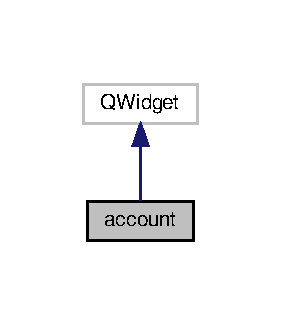
\includegraphics[width=135pt]{classaccount__inherit__graph}
\end{center}
\end{figure}


Collaboration diagram for account\+:
\nopagebreak
\begin{figure}[H]
\begin{center}
\leavevmode
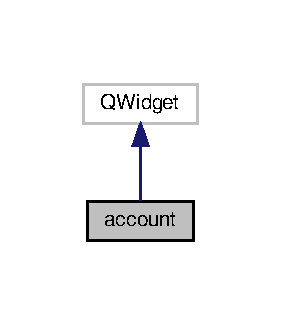
\includegraphics[width=135pt]{classaccount__coll__graph}
\end{center}
\end{figure}
\subsection*{Public Member Functions}
\begin{DoxyCompactItemize}
\item 
\hyperlink{classaccount_a366fd4d75f8c386ea788b0497e8a7cac}{account} (Q\+Widget $\ast$parent=nullptr, Q\+Json\+Object json=\{\})
\begin{DoxyCompactList}\small\item\em account constructor \end{DoxyCompactList}\end{DoxyCompactItemize}


\subsection{Constructor \& Destructor Documentation}
\mbox{\Hypertarget{classaccount_a366fd4d75f8c386ea788b0497e8a7cac}\label{classaccount_a366fd4d75f8c386ea788b0497e8a7cac}} 
\index{account@{account}!account@{account}}
\index{account@{account}!account@{account}}
\subsubsection{\texorpdfstring{account()}{account()}}
{\footnotesize\ttfamily account\+::account (\begin{DoxyParamCaption}\item[{Q\+Widget $\ast$}]{parent = {\ttfamily nullptr},  }\item[{Q\+Json\+Object}]{json = {\ttfamily \{\}} }\end{DoxyParamCaption})\hspace{0.3cm}{\ttfamily [explicit]}}



account constructor 


\begin{DoxyParams}{Parameters}
{\em parent,a} & pointer to a parent widget \\
\hline
{\em Q\+Json\+Object,the} & user json object returned from signin, signup, or playasguest \\
\hline
\end{DoxyParams}


The documentation for this class was generated from the following files\+:\begin{DoxyCompactItemize}
\item 
\hyperlink{account_8h}{account.\+h}\item 
\hyperlink{account_8cpp}{account.\+cpp}\end{DoxyCompactItemize}

\hypertarget{classaccount__dashboard}{}\section{account\+\_\+dashboard Class Reference}
\label{classaccount__dashboard}\index{account\+\_\+dashboard@{account\+\_\+dashboard}}


Inheritance diagram for account\+\_\+dashboard\+:
\nopagebreak
\begin{figure}[H]
\begin{center}
\leavevmode
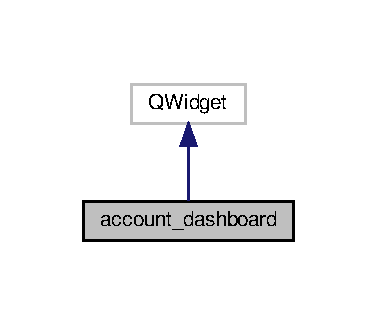
\includegraphics[width=181pt]{classaccount__dashboard__inherit__graph}
\end{center}
\end{figure}


Collaboration diagram for account\+\_\+dashboard\+:
\nopagebreak
\begin{figure}[H]
\begin{center}
\leavevmode
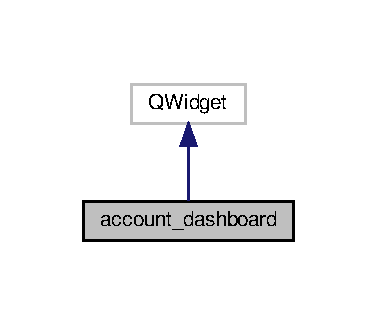
\includegraphics[width=181pt]{classaccount__dashboard__coll__graph}
\end{center}
\end{figure}
\subsection*{Public Member Functions}
\begin{DoxyCompactItemize}
\item 
\hyperlink{classaccount__dashboard_a17892d9c39fe88dd8a645c4cd6a08d26}{account\+\_\+dashboard} (Q\+Widget $\ast$parent=nullptr, Q\+Json\+Object json=\{\}, Q\+String game\+ID=\char`\"{}\char`\"{})
\begin{DoxyCompactList}\small\item\em \hyperlink{classaccount__dashboard}{account\+\_\+dashboard} constructor \end{DoxyCompactList}\end{DoxyCompactItemize}


\subsection{Constructor \& Destructor Documentation}
\mbox{\Hypertarget{classaccount__dashboard_a17892d9c39fe88dd8a645c4cd6a08d26}\label{classaccount__dashboard_a17892d9c39fe88dd8a645c4cd6a08d26}} 
\index{account\+\_\+dashboard@{account\+\_\+dashboard}!account\+\_\+dashboard@{account\+\_\+dashboard}}
\index{account\+\_\+dashboard@{account\+\_\+dashboard}!account\+\_\+dashboard@{account\+\_\+dashboard}}
\subsubsection{\texorpdfstring{account\+\_\+dashboard()}{account\_dashboard()}}
{\footnotesize\ttfamily account\+\_\+dashboard\+::account\+\_\+dashboard (\begin{DoxyParamCaption}\item[{Q\+Widget $\ast$}]{parent = {\ttfamily nullptr},  }\item[{Q\+Json\+Object}]{json = {\ttfamily \{\}},  }\item[{Q\+String}]{game\+ID = {\ttfamily \char`\"{}\char`\"{}} }\end{DoxyParamCaption})\hspace{0.3cm}{\ttfamily [explicit]}}



\hyperlink{classaccount__dashboard}{account\+\_\+dashboard} constructor 


\begin{DoxyParams}{Parameters}
{\em parent,a} & pointer to a parent Q\+Widget. Initially equal to a nullptr \\
\hline
{\em json,a} & user Q\+Json\+Object passed by the calling class. Initialized to an empty object. \\
\hline
{\em game\+ID,a} & Q\+String with the game\textquotesingle{}s ID to differeniate between stats of different games. Initialized to an empty string. \\
\hline
\end{DoxyParams}


The documentation for this class was generated from the following files\+:\begin{DoxyCompactItemize}
\item 
\hyperlink{account__dashboard_8h}{account\+\_\+dashboard.\+h}\item 
\hyperlink{account__dashboard_8cpp}{account\+\_\+dashboard.\+cpp}\end{DoxyCompactItemize}

\hypertarget{classaccount__sidebar}{}\section{account\+\_\+sidebar Class Reference}
\label{classaccount__sidebar}\index{account\+\_\+sidebar@{account\+\_\+sidebar}}


Inheritance diagram for account\+\_\+sidebar\+:
\nopagebreak
\begin{figure}[H]
\begin{center}
\leavevmode
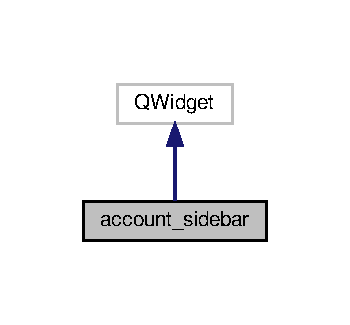
\includegraphics[width=168pt]{classaccount__sidebar__inherit__graph}
\end{center}
\end{figure}


Collaboration diagram for account\+\_\+sidebar\+:
\nopagebreak
\begin{figure}[H]
\begin{center}
\leavevmode
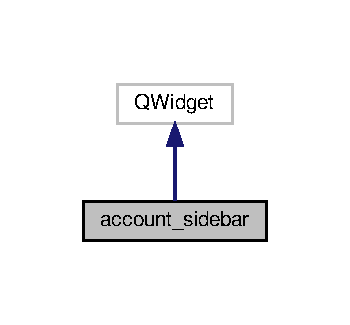
\includegraphics[width=168pt]{classaccount__sidebar__coll__graph}
\end{center}
\end{figure}
\subsection*{Public Member Functions}
\begin{DoxyCompactItemize}
\item 
\hyperlink{classaccount__sidebar_a6fa648be2eabdef0be7b5f27a16ac7f1}{account\+\_\+sidebar} (Q\+Widget $\ast$parent=nullptr, Q\+Json\+Object userobj=\{\})
\begin{DoxyCompactList}\small\item\em \hyperlink{classaccount__sidebar}{account\+\_\+sidebar} constructor \end{DoxyCompactList}\end{DoxyCompactItemize}


\subsection{Constructor \& Destructor Documentation}
\mbox{\Hypertarget{classaccount__sidebar_a6fa648be2eabdef0be7b5f27a16ac7f1}\label{classaccount__sidebar_a6fa648be2eabdef0be7b5f27a16ac7f1}} 
\index{account\+\_\+sidebar@{account\+\_\+sidebar}!account\+\_\+sidebar@{account\+\_\+sidebar}}
\index{account\+\_\+sidebar@{account\+\_\+sidebar}!account\+\_\+sidebar@{account\+\_\+sidebar}}
\subsubsection{\texorpdfstring{account\+\_\+sidebar()}{account\_sidebar()}}
{\footnotesize\ttfamily account\+\_\+sidebar\+::account\+\_\+sidebar (\begin{DoxyParamCaption}\item[{Q\+Widget $\ast$}]{parent = {\ttfamily nullptr},  }\item[{Q\+Json\+Object}]{userobj = {\ttfamily \{\}} }\end{DoxyParamCaption})\hspace{0.3cm}{\ttfamily [explicit]}}



\hyperlink{classaccount__sidebar}{account\+\_\+sidebar} constructor 


\begin{DoxyParams}{Parameters}
{\em parent,a} & pointer to a parent Q\+Widget. Initialized to nullptr \\
\hline
{\em userobj,a} & Q\+Json\+Object. Initialized to an empty Q\+Json\+Object. \\
\hline
\end{DoxyParams}


The documentation for this class was generated from the following files\+:\begin{DoxyCompactItemize}
\item 
\hyperlink{account__sidebar_8h}{account\+\_\+sidebar.\+h}\item 
\hyperlink{account__sidebar_8cpp}{account\+\_\+sidebar.\+cpp}\end{DoxyCompactItemize}

\hypertarget{classbutb}{}\section{butb Class Reference}
\label{classbutb}\index{butb@{butb}}


Inheritance diagram for butb\+:
\nopagebreak
\begin{figure}[H]
\begin{center}
\leavevmode
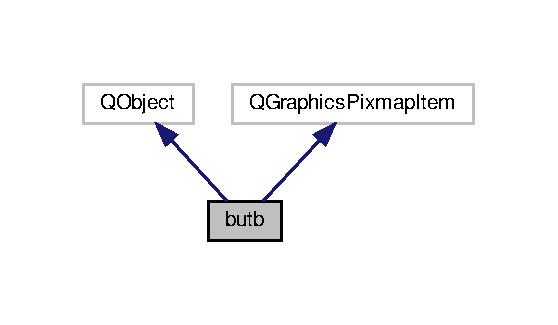
\includegraphics[width=268pt]{classbutb__inherit__graph}
\end{center}
\end{figure}


Collaboration diagram for butb\+:
\nopagebreak
\begin{figure}[H]
\begin{center}
\leavevmode
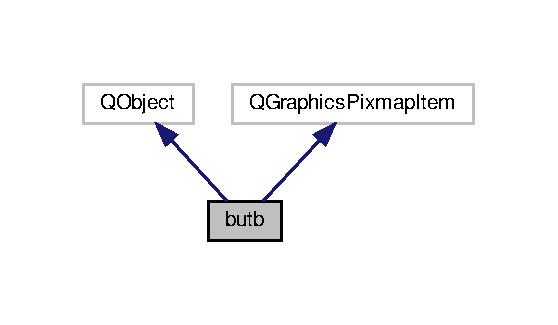
\includegraphics[width=268pt]{classbutb__coll__graph}
\end{center}
\end{figure}
\subsection*{Public Types}
\begin{DoxyCompactItemize}
\item 
\mbox{\Hypertarget{classbutb_a1a07f03f7feef35e03fea73d8d430377}\label{classbutb_a1a07f03f7feef35e03fea73d8d430377}} 
enum {\bfseries Disk\+Type} \{ {\bfseries Black} = User\+Type + 1, 
{\bfseries Blue} = User\+Type + 2, 
{\bfseries Green} = User\+Type + 3, 
{\bfseries Purple} = User\+Type + 4
 \}
\end{DoxyCompactItemize}
\subsection*{Public Member Functions}
\begin{DoxyCompactItemize}
\item 
\hyperlink{classbutb_a8a6a1e82497086cc0cc6fb4732fa5edb}{butb} (Q\+Object $\ast$parent=nullptr, int pos=5)
\begin{DoxyCompactList}\small\item\em butb constructor \end{DoxyCompactList}\item 
\mbox{\Hypertarget{classbutb_a5322fcf31cfb49cc19219a366ec4a56f}\label{classbutb_a5322fcf31cfb49cc19219a366ec4a56f}} 
int {\bfseries type} () const override
\end{DoxyCompactItemize}


\subsection{Constructor \& Destructor Documentation}
\mbox{\Hypertarget{classbutb_a8a6a1e82497086cc0cc6fb4732fa5edb}\label{classbutb_a8a6a1e82497086cc0cc6fb4732fa5edb}} 
\index{butb@{butb}!butb@{butb}}
\index{butb@{butb}!butb@{butb}}
\subsubsection{\texorpdfstring{butb()}{butb()}}
{\footnotesize\ttfamily butb\+::butb (\begin{DoxyParamCaption}\item[{Q\+Object $\ast$}]{parent = {\ttfamily nullptr},  }\item[{int}]{pos = {\ttfamily 5} }\end{DoxyParamCaption})\hspace{0.3cm}{\ttfamily [explicit]}}



butb constructor 


\begin{DoxyParams}{Parameters}
{\em parent,a} & pointer to a parent Q\+Object, initialized to a nullptr \\
\hline
{\em pos,position} & by which the button falls \\
\hline
\end{DoxyParams}


The documentation for this class was generated from the following files\+:\begin{DoxyCompactItemize}
\item 
\hyperlink{butb_8h}{butb.\+h}\item 
\hyperlink{butb_8cpp}{butb.\+cpp}\end{DoxyCompactItemize}

\hypertarget{classbutblack}{}\section{butblack Class Reference}
\label{classbutblack}\index{butblack@{butblack}}


Inheritance diagram for butblack\+:
\nopagebreak
\begin{figure}[H]
\begin{center}
\leavevmode
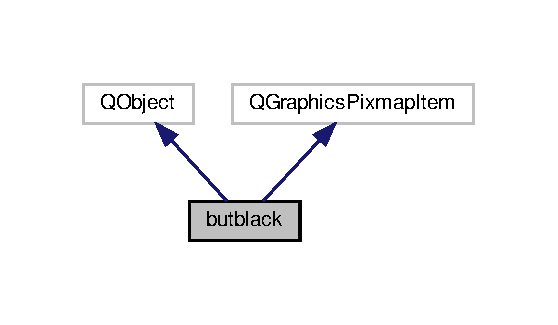
\includegraphics[width=268pt]{classbutblack__inherit__graph}
\end{center}
\end{figure}


Collaboration diagram for butblack\+:
\nopagebreak
\begin{figure}[H]
\begin{center}
\leavevmode
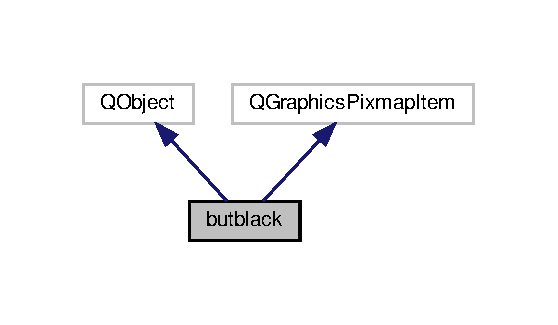
\includegraphics[width=268pt]{classbutblack__coll__graph}
\end{center}
\end{figure}
\subsection*{Public Types}
\begin{DoxyCompactItemize}
\item 
\mbox{\Hypertarget{classbutblack_ad799fb56af60a3269b1505a34701ebae}\label{classbutblack_ad799fb56af60a3269b1505a34701ebae}} 
enum {\bfseries Disk\+Type} \{ {\bfseries Black} = User\+Type + 1, 
{\bfseries Blue} = User\+Type + 2, 
{\bfseries Green} = User\+Type + 3, 
{\bfseries Purple} = User\+Type + 4
 \}
\end{DoxyCompactItemize}
\subsection*{Public Member Functions}
\begin{DoxyCompactItemize}
\item 
\hyperlink{classbutblack_a21b44428bac698691a86f593ce6bc887}{butblack} (Q\+Object $\ast$parent=nullptr, int x=0, int pos=5)
\begin{DoxyCompactList}\small\item\em butblack constructor \end{DoxyCompactList}\item 
\mbox{\Hypertarget{classbutblack_a73504f75bb64f8c4c605c6f4384d7ce2}\label{classbutblack_a73504f75bb64f8c4c605c6f4384d7ce2}} 
int {\bfseries type} () const override
\end{DoxyCompactItemize}


\subsection{Constructor \& Destructor Documentation}
\mbox{\Hypertarget{classbutblack_a21b44428bac698691a86f593ce6bc887}\label{classbutblack_a21b44428bac698691a86f593ce6bc887}} 
\index{butblack@{butblack}!butblack@{butblack}}
\index{butblack@{butblack}!butblack@{butblack}}
\subsubsection{\texorpdfstring{butblack()}{butblack()}}
{\footnotesize\ttfamily butblack\+::butblack (\begin{DoxyParamCaption}\item[{Q\+Object $\ast$}]{parent = {\ttfamily nullptr},  }\item[{int}]{x = {\ttfamily 0},  }\item[{int}]{pos = {\ttfamily 5} }\end{DoxyParamCaption})\hspace{0.3cm}{\ttfamily [explicit]}}



butblack constructor 

butb constructor


\begin{DoxyParams}{Parameters}
{\em parent,a} & pointer to a parent Q\+Object, initialized to a nullptr \\
\hline
{\em x,the} & x coordinate at which the grey button should fall \\
\hline
{\em pos,position} & by which the button falls \\
\hline
\end{DoxyParams}


The documentation for this class was generated from the following files\+:\begin{DoxyCompactItemize}
\item 
\hyperlink{butblack_8h}{butblack.\+h}\item 
\hyperlink{butblack_8cpp}{butblack.\+cpp}\end{DoxyCompactItemize}

\hypertarget{classbutg}{}\section{butg Class Reference}
\label{classbutg}\index{butg@{butg}}


Inheritance diagram for butg\+:
\nopagebreak
\begin{figure}[H]
\begin{center}
\leavevmode
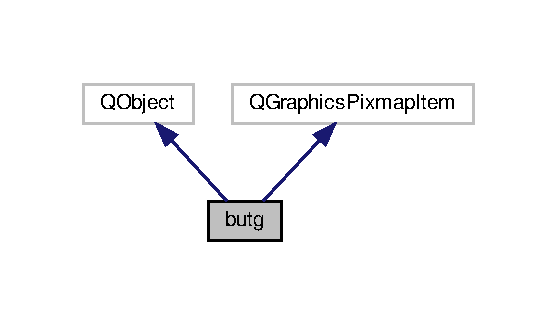
\includegraphics[width=268pt]{classbutg__inherit__graph}
\end{center}
\end{figure}


Collaboration diagram for butg\+:
\nopagebreak
\begin{figure}[H]
\begin{center}
\leavevmode
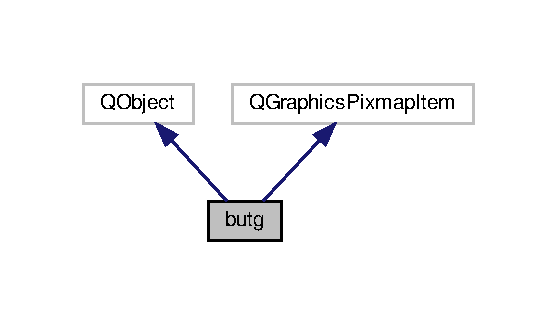
\includegraphics[width=268pt]{classbutg__coll__graph}
\end{center}
\end{figure}
\subsection*{Public Types}
\begin{DoxyCompactItemize}
\item 
\mbox{\Hypertarget{classbutg_adff525298cdca0bcfa0929c361f6600d}\label{classbutg_adff525298cdca0bcfa0929c361f6600d}} 
enum {\bfseries Disk\+Type} \{ {\bfseries Black} = User\+Type + 1, 
{\bfseries Blue} = User\+Type + 2, 
{\bfseries Green} = User\+Type + 3, 
{\bfseries Purple} = User\+Type + 4
 \}
\end{DoxyCompactItemize}
\subsection*{Public Member Functions}
\begin{DoxyCompactItemize}
\item 
\hyperlink{classbutg_a814505efd430ff6986a6f0b5eccd9fc0}{butg} (Q\+Object $\ast$parent=nullptr, int pos=5)
\begin{DoxyCompactList}\small\item\em butg constructor \end{DoxyCompactList}\item 
\mbox{\Hypertarget{classbutg_a2b7419db95240dccc8172c1b192b876e}\label{classbutg_a2b7419db95240dccc8172c1b192b876e}} 
int {\bfseries type} () const override
\end{DoxyCompactItemize}


\subsection{Constructor \& Destructor Documentation}
\mbox{\Hypertarget{classbutg_a814505efd430ff6986a6f0b5eccd9fc0}\label{classbutg_a814505efd430ff6986a6f0b5eccd9fc0}} 
\index{butg@{butg}!butg@{butg}}
\index{butg@{butg}!butg@{butg}}
\subsubsection{\texorpdfstring{butg()}{butg()}}
{\footnotesize\ttfamily butg\+::butg (\begin{DoxyParamCaption}\item[{Q\+Object $\ast$}]{parent = {\ttfamily nullptr},  }\item[{int}]{pos = {\ttfamily 5} }\end{DoxyParamCaption})\hspace{0.3cm}{\ttfamily [explicit]}}



butg constructor 


\begin{DoxyParams}{Parameters}
{\em parent,a} & pointer to a parent Q\+Object, initialized to a nullptr \\
\hline
{\em x,the} & x coordinate at which the grey button should fall \\
\hline
{\em pos,position} & by which the button falls \\
\hline
\end{DoxyParams}


The documentation for this class was generated from the following files\+:\begin{DoxyCompactItemize}
\item 
\hyperlink{butg_8h}{butg.\+h}\item 
\hyperlink{butg_8cpp}{butg.\+cpp}\end{DoxyCompactItemize}

\hypertarget{classbutp}{}\section{butp Class Reference}
\label{classbutp}\index{butp@{butp}}


Inheritance diagram for butp\+:
\nopagebreak
\begin{figure}[H]
\begin{center}
\leavevmode
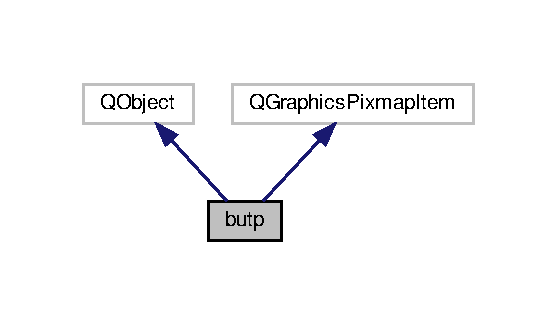
\includegraphics[width=268pt]{classbutp__inherit__graph}
\end{center}
\end{figure}


Collaboration diagram for butp\+:
\nopagebreak
\begin{figure}[H]
\begin{center}
\leavevmode
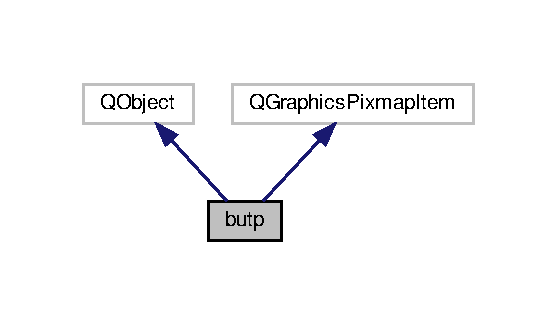
\includegraphics[width=268pt]{classbutp__coll__graph}
\end{center}
\end{figure}
\subsection*{Public Types}
\begin{DoxyCompactItemize}
\item 
\mbox{\Hypertarget{classbutp_a5da9f507b30a431c244aca25cd0418f0}\label{classbutp_a5da9f507b30a431c244aca25cd0418f0}} 
enum {\bfseries Disk\+Type} \{ {\bfseries Black} = User\+Type + 1, 
{\bfseries Blue} = User\+Type + 2, 
{\bfseries Green} = User\+Type + 3, 
{\bfseries Purple} = User\+Type + 4
 \}
\end{DoxyCompactItemize}
\subsection*{Public Member Functions}
\begin{DoxyCompactItemize}
\item 
\hyperlink{classbutp_abfdbf8481fc25fa88cf2d29b68163041}{butp} (Q\+Object $\ast$parent=nullptr, int pos=5)
\begin{DoxyCompactList}\small\item\em butp constructor \end{DoxyCompactList}\item 
\mbox{\Hypertarget{classbutp_a4971613be174a28767e439bc46f464c8}\label{classbutp_a4971613be174a28767e439bc46f464c8}} 
int {\bfseries type} () const override
\end{DoxyCompactItemize}


\subsection{Constructor \& Destructor Documentation}
\mbox{\Hypertarget{classbutp_abfdbf8481fc25fa88cf2d29b68163041}\label{classbutp_abfdbf8481fc25fa88cf2d29b68163041}} 
\index{butp@{butp}!butp@{butp}}
\index{butp@{butp}!butp@{butp}}
\subsubsection{\texorpdfstring{butp()}{butp()}}
{\footnotesize\ttfamily butp\+::butp (\begin{DoxyParamCaption}\item[{Q\+Object $\ast$}]{parent = {\ttfamily nullptr},  }\item[{int}]{pos = {\ttfamily 5} }\end{DoxyParamCaption})\hspace{0.3cm}{\ttfamily [explicit]}}



butp constructor 


\begin{DoxyParams}{Parameters}
{\em parent,a} & pointer to a parent Q\+Object, initialized to a nullptr \\
\hline
{\em pos,position} & by which the button falls \\
\hline
\end{DoxyParams}


The documentation for this class was generated from the following files\+:\begin{DoxyCompactItemize}
\item 
\hyperlink{butp_8h}{butp.\+h}\item 
\hyperlink{butp_8cpp}{butp.\+cpp}\end{DoxyCompactItemize}

\hypertarget{classCentering}{}\section{Centering Class Reference}
\label{classCentering}\index{Centering@{Centering}}


Inheritance diagram for Centering\+:
\nopagebreak
\begin{figure}[H]
\begin{center}
\leavevmode
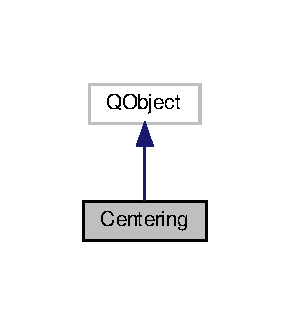
\includegraphics[width=139pt]{classCentering__inherit__graph}
\end{center}
\end{figure}


Collaboration diagram for Centering\+:
\nopagebreak
\begin{figure}[H]
\begin{center}
\leavevmode
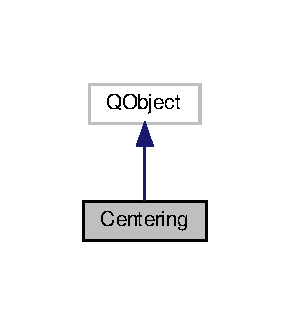
\includegraphics[width=139pt]{classCentering__coll__graph}
\end{center}
\end{figure}
\subsection*{Public Member Functions}
\begin{DoxyCompactItemize}
\item 
\hyperlink{classCentering_a7b09cff0f47876166f14d3f9ced073e3}{Centering} (Q\+Object $\ast$parent=nullptr)
\begin{DoxyCompactList}\small\item\em \hyperlink{classCentering}{Centering} constructor. \end{DoxyCompactList}\end{DoxyCompactItemize}
\subsection*{Static Public Member Functions}
\begin{DoxyCompactItemize}
\item 
static void \hyperlink{classCentering_a74aff632edb0a6587ac20b8974026f26}{center\+Widget} (Q\+Widget $\ast$w)
\begin{DoxyCompactList}\small\item\em a function that centers a widget \end{DoxyCompactList}\item 
\mbox{\Hypertarget{classCentering_a400ac287c7c0a1a7c08ebedc16d8c123}\label{classCentering_a400ac287c7c0a1a7c08ebedc16d8c123}} 
static void {\bfseries center\+Scene} (Q\+Graphics\+View $\ast$s)
\end{DoxyCompactItemize}


\subsection{Constructor \& Destructor Documentation}
\mbox{\Hypertarget{classCentering_a7b09cff0f47876166f14d3f9ced073e3}\label{classCentering_a7b09cff0f47876166f14d3f9ced073e3}} 
\index{Centering@{Centering}!Centering@{Centering}}
\index{Centering@{Centering}!Centering@{Centering}}
\subsubsection{\texorpdfstring{Centering()}{Centering()}}
{\footnotesize\ttfamily Centering\+::\+Centering (\begin{DoxyParamCaption}\item[{Q\+Object $\ast$}]{parent = {\ttfamily nullptr} }\end{DoxyParamCaption})\hspace{0.3cm}{\ttfamily [explicit]}}



\hyperlink{classCentering}{Centering} constructor. 


\begin{DoxyParams}{Parameters}
{\em parent,a} & pointer to parent Q\+Object. Initialized to a nullptr \\
\hline
\end{DoxyParams}


\subsection{Member Function Documentation}
\mbox{\Hypertarget{classCentering_a74aff632edb0a6587ac20b8974026f26}\label{classCentering_a74aff632edb0a6587ac20b8974026f26}} 
\index{Centering@{Centering}!center\+Widget@{center\+Widget}}
\index{center\+Widget@{center\+Widget}!Centering@{Centering}}
\subsubsection{\texorpdfstring{center\+Widget()}{centerWidget()}}
{\footnotesize\ttfamily void Centering\+::center\+Widget (\begin{DoxyParamCaption}\item[{Q\+Widget $\ast$}]{w }\end{DoxyParamCaption})\hspace{0.3cm}{\ttfamily [static]}}



a function that centers a widget 


\begin{DoxyParams}{Parameters}
{\em w,a} & pointer to the Q\+Widget to be centered \\
\hline
\end{DoxyParams}


The documentation for this class was generated from the following files\+:\begin{DoxyCompactItemize}
\item 
centering.\+h\item 
centering.\+cpp\end{DoxyCompactItemize}

\hypertarget{classg1__info}{}\section{g1\+\_\+info Class Reference}
\label{classg1__info}\index{g1\+\_\+info@{g1\+\_\+info}}


Inheritance diagram for g1\+\_\+info\+:
\nopagebreak
\begin{figure}[H]
\begin{center}
\leavevmode
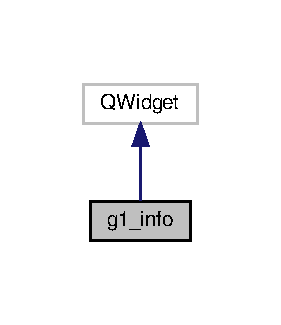
\includegraphics[width=135pt]{classg1__info__inherit__graph}
\end{center}
\end{figure}


Collaboration diagram for g1\+\_\+info\+:
\nopagebreak
\begin{figure}[H]
\begin{center}
\leavevmode
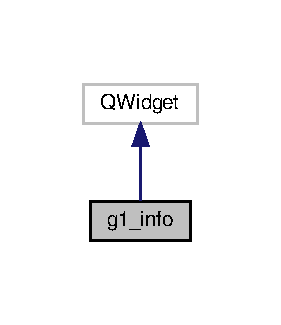
\includegraphics[width=135pt]{classg1__info__coll__graph}
\end{center}
\end{figure}
\subsection*{Public Member Functions}
\begin{DoxyCompactItemize}
\item 
\hyperlink{classg1__info_ae492d616a5f3dd0dc3177fdae814288d}{g1\+\_\+info} (Q\+Widget $\ast$parent=nullptr, Q\+Json\+Object json=\{\})
\begin{DoxyCompactList}\small\item\em \hyperlink{classg1__info}{g1\+\_\+info} constructor \end{DoxyCompactList}\end{DoxyCompactItemize}


\subsection{Constructor \& Destructor Documentation}
\mbox{\Hypertarget{classg1__info_ae492d616a5f3dd0dc3177fdae814288d}\label{classg1__info_ae492d616a5f3dd0dc3177fdae814288d}} 
\index{g1\+\_\+info@{g1\+\_\+info}!g1\+\_\+info@{g1\+\_\+info}}
\index{g1\+\_\+info@{g1\+\_\+info}!g1\+\_\+info@{g1\+\_\+info}}
\subsubsection{\texorpdfstring{g1\+\_\+info()}{g1\_info()}}
{\footnotesize\ttfamily g1\+\_\+info\+::g1\+\_\+info (\begin{DoxyParamCaption}\item[{Q\+Widget $\ast$}]{parent = {\ttfamily nullptr},  }\item[{Q\+Json\+Object}]{json = {\ttfamily \{\}} }\end{DoxyParamCaption})\hspace{0.3cm}{\ttfamily [explicit]}}



\hyperlink{classg1__info}{g1\+\_\+info} constructor 


\begin{DoxyParams}{Parameters}
{\em parent,a} & pointer to a Q\+Widget parent \\
\hline
{\em json,the} & Q\+Json\+Object for a given user \\
\hline
\end{DoxyParams}


The documentation for this class was generated from the following files\+:\begin{DoxyCompactItemize}
\item 
\hyperlink{g1__info_8h}{g1\+\_\+info.\+h}\item 
\hyperlink{g1__info_8cpp}{g1\+\_\+info.\+cpp}\end{DoxyCompactItemize}

\hypertarget{classg1__settings}{}\section{g1\+\_\+settings Class Reference}
\label{classg1__settings}\index{g1\+\_\+settings@{g1\+\_\+settings}}


Inheritance diagram for g1\+\_\+settings\+:
\nopagebreak
\begin{figure}[H]
\begin{center}
\leavevmode
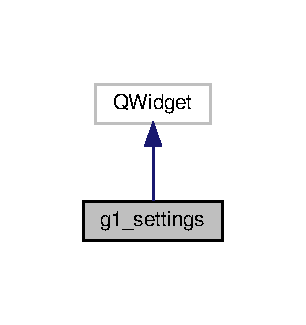
\includegraphics[width=147pt]{classg1__settings__inherit__graph}
\end{center}
\end{figure}


Collaboration diagram for g1\+\_\+settings\+:
\nopagebreak
\begin{figure}[H]
\begin{center}
\leavevmode
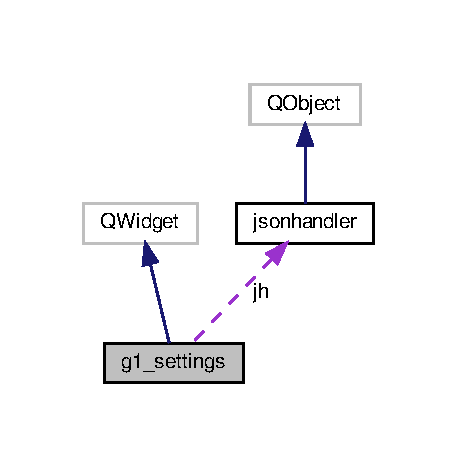
\includegraphics[width=220pt]{classg1__settings__coll__graph}
\end{center}
\end{figure}
\subsection*{Public Member Functions}
\begin{DoxyCompactItemize}
\item 
\hyperlink{classg1__settings_a0528bafcafa9832b59f045b59e1ab260}{g1\+\_\+settings} (Q\+Widget $\ast$parent=nullptr, Q\+Json\+Object json=\{\})
\begin{DoxyCompactList}\small\item\em \hyperlink{classg1__settings}{g1\+\_\+settings} constructor \end{DoxyCompactList}\item 
\mbox{\Hypertarget{classg1__settings_af7571badf3ba81ae73f94fcdcbf00972}\label{classg1__settings_af7571badf3ba81ae73f94fcdcbf00972}} 
void \hyperlink{classg1__settings_af7571badf3ba81ae73f94fcdcbf00972}{set\+Grid\+Layout} ()
\begin{DoxyCompactList}\small\item\em Sets the widget of the grid layout. \end{DoxyCompactList}\item 
\mbox{\Hypertarget{classg1__settings_a5b1b70cf0a14c23ec8af63b1a68b6caf}\label{classg1__settings_a5b1b70cf0a14c23ec8af63b1a68b6caf}} 
void \hyperlink{classg1__settings_a5b1b70cf0a14c23ec8af63b1a68b6caf}{create\+Difficulty\+Box} ()
\begin{DoxyCompactList}\small\item\em groups the difficulty buttons \end{DoxyCompactList}\item 
\mbox{\Hypertarget{classg1__settings_aa99a57bac7a673e2bd59b739c35808f1}\label{classg1__settings_aa99a57bac7a673e2bd59b739c35808f1}} 
void \hyperlink{classg1__settings_aa99a57bac7a673e2bd59b739c35808f1}{create\+Topic\+Box} ()
\begin{DoxyCompactList}\small\item\em groups the topic buttons \end{DoxyCompactList}\item 
\mbox{\Hypertarget{classg1__settings_a1a024dbe1251bfabd6a4ff5691b4586e}\label{classg1__settings_a1a024dbe1251bfabd6a4ff5691b4586e}} 
void \hyperlink{classg1__settings_a1a024dbe1251bfabd6a4ff5691b4586e}{create\+Bg\+Box} ()
\begin{DoxyCompactList}\small\item\em groups the background buttons \end{DoxyCompactList}\item 
\mbox{\Hypertarget{classg1__settings_af75c3f57731ff8ced7e439328df3eddb}\label{classg1__settings_af75c3f57731ff8ced7e439328df3eddb}} 
void \hyperlink{classg1__settings_af75c3f57731ff8ced7e439328df3eddb}{init\+Bg} ()
\begin{DoxyCompactList}\small\item\em initializes the background color of the Q\+Widget as specified in user\+Json. \end{DoxyCompactList}\end{DoxyCompactItemize}
\subsection*{Public Attributes}
\begin{DoxyCompactItemize}
\item 
\mbox{\Hypertarget{classg1__settings_a3d371dbb7b74cf6f2ff29f14ea0db3bb}\label{classg1__settings_a3d371dbb7b74cf6f2ff29f14ea0db3bb}} 
Q\+Push\+Button $\ast$ {\bfseries back\+Btn}
\item 
\mbox{\Hypertarget{classg1__settings_a02d31ba0d8c4a89a4a6849c07a359564}\label{classg1__settings_a02d31ba0d8c4a89a4a6849c07a359564}} 
Q\+Label $\ast$ {\bfseries title}
\item 
\mbox{\Hypertarget{classg1__settings_aab4364dba79b531ec648879f8b3690ed}\label{classg1__settings_aab4364dba79b531ec648879f8b3690ed}} 
Q\+Label $\ast$ {\bfseries diff\+Label}
\item 
\mbox{\Hypertarget{classg1__settings_a10ed8152748aaab49c44db3429413026}\label{classg1__settings_a10ed8152748aaab49c44db3429413026}} 
Q\+Label $\ast$ {\bfseries topic\+Label}
\item 
\mbox{\Hypertarget{classg1__settings_aa3a62b3e757280b9094c32c13cd458df}\label{classg1__settings_aa3a62b3e757280b9094c32c13cd458df}} 
Q\+Label $\ast$ {\bfseries bg\+Label}
\item 
\mbox{\Hypertarget{classg1__settings_aaa32a6f663f09f70833c87d3c3d012df}\label{classg1__settings_aaa32a6f663f09f70833c87d3c3d012df}} 
Q\+Push\+Button $\ast$ {\bfseries easy\+Btn}
\item 
\mbox{\Hypertarget{classg1__settings_a9f7a5d53e935d15fa2c1e50aba1cc326}\label{classg1__settings_a9f7a5d53e935d15fa2c1e50aba1cc326}} 
Q\+Push\+Button $\ast$ {\bfseries medium\+Btn}
\item 
\mbox{\Hypertarget{classg1__settings_a59c7d2f1da102bf75975d205804b6530}\label{classg1__settings_a59c7d2f1da102bf75975d205804b6530}} 
Q\+Push\+Button $\ast$ {\bfseries hard\+Btn}
\item 
\mbox{\Hypertarget{classg1__settings_ac9d8d652b606c03a06e90cc5fc23e216}\label{classg1__settings_ac9d8d652b606c03a06e90cc5fc23e216}} 
Q\+Group\+Box $\ast$ {\bfseries difficulty\+Box}
\item 
\mbox{\Hypertarget{classg1__settings_a9cf96e6fc0e07b763fc4eac1edf754ce}\label{classg1__settings_a9cf96e6fc0e07b763fc4eac1edf754ce}} 
Q\+H\+Box\+Layout $\ast$ {\bfseries diff\+Box\+Layout}
\item 
\mbox{\Hypertarget{classg1__settings_acbafaeca455e2dfb3981d128c4cb033f}\label{classg1__settings_acbafaeca455e2dfb3981d128c4cb033f}} 
Q\+Push\+Button $\ast$ {\bfseries t1\+Btn}
\item 
\mbox{\Hypertarget{classg1__settings_aa944758a294099c7376939b47e159ffa}\label{classg1__settings_aa944758a294099c7376939b47e159ffa}} 
Q\+Push\+Button $\ast$ {\bfseries t2\+Btn}
\item 
\mbox{\Hypertarget{classg1__settings_a7e8211d3e45f5c436ced139f39214859}\label{classg1__settings_a7e8211d3e45f5c436ced139f39214859}} 
Q\+Push\+Button $\ast$ {\bfseries t3\+Btn}
\item 
\mbox{\Hypertarget{classg1__settings_a344e4a24c172591f69216bb08699288a}\label{classg1__settings_a344e4a24c172591f69216bb08699288a}} 
Q\+Group\+Box $\ast$ {\bfseries topic\+Box}
\item 
\mbox{\Hypertarget{classg1__settings_ac9a6fa417d9844cf50ff4973bbbe9677}\label{classg1__settings_ac9a6fa417d9844cf50ff4973bbbe9677}} 
Q\+H\+Box\+Layout $\ast$ {\bfseries topic\+Box\+Layout}
\item 
\mbox{\Hypertarget{classg1__settings_a839020acfd551c2c959401f796bb330b}\label{classg1__settings_a839020acfd551c2c959401f796bb330b}} 
Q\+Push\+Button $\ast$ {\bfseries bg1\+Btn}
\item 
\mbox{\Hypertarget{classg1__settings_aceea6ab2c98e77a8bcdc33dc048a4066}\label{classg1__settings_aceea6ab2c98e77a8bcdc33dc048a4066}} 
Q\+Push\+Button $\ast$ {\bfseries bg2\+Btn}
\item 
\mbox{\Hypertarget{classg1__settings_a1fda77309f20856876b7ac445c17d8f3}\label{classg1__settings_a1fda77309f20856876b7ac445c17d8f3}} 
Q\+Push\+Button $\ast$ {\bfseries bg3\+Btn}
\item 
\mbox{\Hypertarget{classg1__settings_ab1184f542509b44f21b3b250c640cb59}\label{classg1__settings_ab1184f542509b44f21b3b250c640cb59}} 
Q\+Group\+Box $\ast$ {\bfseries bg\+Box}
\item 
\mbox{\Hypertarget{classg1__settings_a7e51c7bc608d4ecf4e1201794a4d391c}\label{classg1__settings_a7e51c7bc608d4ecf4e1201794a4d391c}} 
Q\+H\+Box\+Layout $\ast$ {\bfseries bg\+Box\+Layout}
\item 
\mbox{\Hypertarget{classg1__settings_a2c5a6c03e4beee3dcac5ebf101452649}\label{classg1__settings_a2c5a6c03e4beee3dcac5ebf101452649}} 
Q\+Grid\+Layout $\ast$ {\bfseries grid}
\item 
\mbox{\Hypertarget{classg1__settings_a37b7448a79081797d2f3a2a15e183bb7}\label{classg1__settings_a37b7448a79081797d2f3a2a15e183bb7}} 
Q\+Json\+Object {\bfseries user\+Json}
\item 
\mbox{\Hypertarget{classg1__settings_a116b00d120216a239d6706997b456b62}\label{classg1__settings_a116b00d120216a239d6706997b456b62}} 
\hyperlink{classjsonhandler}{jsonhandler} $\ast$ {\bfseries jh} = new \hyperlink{classjsonhandler}{jsonhandler}()
\end{DoxyCompactItemize}


\subsection{Constructor \& Destructor Documentation}
\mbox{\Hypertarget{classg1__settings_a0528bafcafa9832b59f045b59e1ab260}\label{classg1__settings_a0528bafcafa9832b59f045b59e1ab260}} 
\index{g1\+\_\+settings@{g1\+\_\+settings}!g1\+\_\+settings@{g1\+\_\+settings}}
\index{g1\+\_\+settings@{g1\+\_\+settings}!g1\+\_\+settings@{g1\+\_\+settings}}
\subsubsection{\texorpdfstring{g1\+\_\+settings()}{g1\_settings()}}
{\footnotesize\ttfamily g1\+\_\+settings\+::g1\+\_\+settings (\begin{DoxyParamCaption}\item[{Q\+Widget $\ast$}]{parent = {\ttfamily nullptr},  }\item[{Q\+Json\+Object}]{json = {\ttfamily \{\}} }\end{DoxyParamCaption})\hspace{0.3cm}{\ttfamily [explicit]}}



\hyperlink{classg1__settings}{g1\+\_\+settings} constructor 


\begin{DoxyParams}{Parameters}
{\em parent,a} & pointer to a parent Q\+Widget, initialized to a nullptr \\
\hline
{\em json,the} & player\textquotesingle{}s Q\+Json\+Object, initialized to an empty json object \\
\hline
\end{DoxyParams}


The documentation for this class was generated from the following files\+:\begin{DoxyCompactItemize}
\item 
\hyperlink{g1__settings_8h}{g1\+\_\+settings.\+h}\item 
g1\+\_\+settings.\+cpp\end{DoxyCompactItemize}

\hypertarget{classg1__setup}{}\section{g1\+\_\+setup Class Reference}
\label{classg1__setup}\index{g1\+\_\+setup@{g1\+\_\+setup}}


Inheritance diagram for g1\+\_\+setup\+:
\nopagebreak
\begin{figure}[H]
\begin{center}
\leavevmode
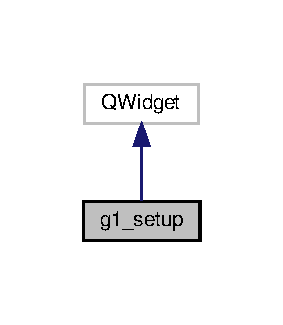
\includegraphics[width=136pt]{classg1__setup__inherit__graph}
\end{center}
\end{figure}


Collaboration diagram for g1\+\_\+setup\+:
\nopagebreak
\begin{figure}[H]
\begin{center}
\leavevmode
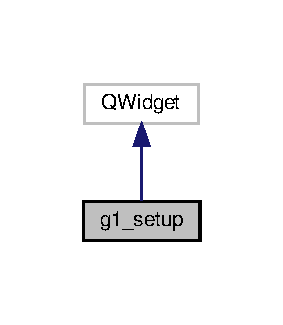
\includegraphics[width=136pt]{classg1__setup__coll__graph}
\end{center}
\end{figure}
\subsection*{Public Member Functions}
\begin{DoxyCompactItemize}
\item 
\hyperlink{classg1__setup_a3ccf5f574bca392284f9c3ae58612162}{g1\+\_\+setup} (Q\+Widget $\ast$parent=nullptr, Q\+Json\+Object json=\{\})
\begin{DoxyCompactList}\small\item\em \hyperlink{classg1__setup}{g1\+\_\+setup} constructor \end{DoxyCompactList}\end{DoxyCompactItemize}


\subsection{Constructor \& Destructor Documentation}
\mbox{\Hypertarget{classg1__setup_a3ccf5f574bca392284f9c3ae58612162}\label{classg1__setup_a3ccf5f574bca392284f9c3ae58612162}} 
\index{g1\+\_\+setup@{g1\+\_\+setup}!g1\+\_\+setup@{g1\+\_\+setup}}
\index{g1\+\_\+setup@{g1\+\_\+setup}!g1\+\_\+setup@{g1\+\_\+setup}}
\subsubsection{\texorpdfstring{g1\+\_\+setup()}{g1\_setup()}}
{\footnotesize\ttfamily g1\+\_\+setup\+::g1\+\_\+setup (\begin{DoxyParamCaption}\item[{Q\+Widget $\ast$}]{parent = {\ttfamily nullptr},  }\item[{Q\+Json\+Object}]{json = {\ttfamily \{\}} }\end{DoxyParamCaption})\hspace{0.3cm}{\ttfamily [explicit]}}



\hyperlink{classg1__setup}{g1\+\_\+setup} constructor 


\begin{DoxyParams}{Parameters}
{\em parent,a} & pointer to a parent Q\+Widget, initialized to a nullptr \\
\hline
{\em json,the} & player\textquotesingle{}s Q\+Json\+Object, initialized to an empty json object \\
\hline
\end{DoxyParams}


The documentation for this class was generated from the following files\+:\begin{DoxyCompactItemize}
\item 
g1\+\_\+setup.\+h\item 
g1\+\_\+setup.\+cpp\end{DoxyCompactItemize}

\hypertarget{classg1__startmenu}{}\section{g1\+\_\+startmenu Class Reference}
\label{classg1__startmenu}\index{g1\+\_\+startmenu@{g1\+\_\+startmenu}}


Inheritance diagram for g1\+\_\+startmenu\+:
\nopagebreak
\begin{figure}[H]
\begin{center}
\leavevmode
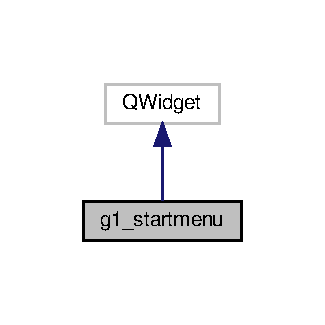
\includegraphics[width=156pt]{classg1__startmenu__inherit__graph}
\end{center}
\end{figure}


Collaboration diagram for g1\+\_\+startmenu\+:
\nopagebreak
\begin{figure}[H]
\begin{center}
\leavevmode
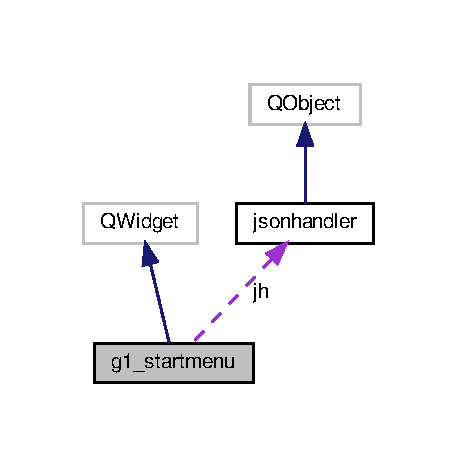
\includegraphics[width=220pt]{classg1__startmenu__coll__graph}
\end{center}
\end{figure}
\subsection*{Public Member Functions}
\begin{DoxyCompactItemize}
\item 
\hyperlink{classg1__startmenu_a85efd01ba5b2843e490b702a1aef8f67}{g1\+\_\+startmenu} (Q\+Widget $\ast$parent=nullptr, Q\+Json\+Object json=\{\})
\begin{DoxyCompactList}\small\item\em \hyperlink{classg1__startmenu}{g1\+\_\+startmenu} constructor \end{DoxyCompactList}\item 
\mbox{\Hypertarget{classg1__startmenu_a96cff080e23c1f6e7d75f0b47fe24800}\label{classg1__startmenu_a96cff080e23c1f6e7d75f0b47fe24800}} 
void \hyperlink{classg1__startmenu_a96cff080e23c1f6e7d75f0b47fe24800}{init\+Bg} ()
\begin{DoxyCompactList}\small\item\em initializes the background color of the Q\+Widget as specified in user\+Json. \end{DoxyCompactList}\end{DoxyCompactItemize}
\subsection*{Public Attributes}
\begin{DoxyCompactItemize}
\item 
\mbox{\Hypertarget{classg1__startmenu_af39d038c880f2d60b7a8e4a2785faeb4}\label{classg1__startmenu_af39d038c880f2d60b7a8e4a2785faeb4}} 
Q\+Push\+Button $\ast$ {\bfseries play\+Btn}
\item 
\mbox{\Hypertarget{classg1__startmenu_a8ec350993f5096be76ad481808025b21}\label{classg1__startmenu_a8ec350993f5096be76ad481808025b21}} 
Q\+Push\+Button $\ast$ {\bfseries settings\+Btn}
\item 
\mbox{\Hypertarget{classg1__startmenu_a526f72b8dc747f347b2c31c55166250b}\label{classg1__startmenu_a526f72b8dc747f347b2c31c55166250b}} 
Q\+Push\+Button $\ast$ {\bfseries exit\+Btn}
\item 
\mbox{\Hypertarget{classg1__startmenu_a10b3391a59fa86be94f89987a16a22da}\label{classg1__startmenu_a10b3391a59fa86be94f89987a16a22da}} 
Q\+Label $\ast$ {\bfseries game\+Logo}
\item 
\mbox{\Hypertarget{classg1__startmenu_a4ff85a91adfdd0b0937da42bba4575c3}\label{classg1__startmenu_a4ff85a91adfdd0b0937da42bba4575c3}} 
Q\+V\+Box\+Layout $\ast$ {\bfseries v\+Layout}
\item 
\mbox{\Hypertarget{classg1__startmenu_ad9784249c69bcdc1e1200e1b44f01800}\label{classg1__startmenu_ad9784249c69bcdc1e1200e1b44f01800}} 
Q\+Json\+Object {\bfseries user\+Json}
\item 
\mbox{\Hypertarget{classg1__startmenu_af6590c97835676c09579e42f34cc34a3}\label{classg1__startmenu_af6590c97835676c09579e42f34cc34a3}} 
\hyperlink{classjsonhandler}{jsonhandler} $\ast$ {\bfseries jh} = new \hyperlink{classjsonhandler}{jsonhandler}()
\end{DoxyCompactItemize}


\subsection{Constructor \& Destructor Documentation}
\mbox{\Hypertarget{classg1__startmenu_a85efd01ba5b2843e490b702a1aef8f67}\label{classg1__startmenu_a85efd01ba5b2843e490b702a1aef8f67}} 
\index{g1\+\_\+startmenu@{g1\+\_\+startmenu}!g1\+\_\+startmenu@{g1\+\_\+startmenu}}
\index{g1\+\_\+startmenu@{g1\+\_\+startmenu}!g1\+\_\+startmenu@{g1\+\_\+startmenu}}
\subsubsection{\texorpdfstring{g1\+\_\+startmenu()}{g1\_startmenu()}}
{\footnotesize\ttfamily g1\+\_\+startmenu\+::g1\+\_\+startmenu (\begin{DoxyParamCaption}\item[{Q\+Widget $\ast$}]{parent = {\ttfamily nullptr},  }\item[{Q\+Json\+Object}]{json = {\ttfamily \{\}} }\end{DoxyParamCaption})\hspace{0.3cm}{\ttfamily [explicit]}}



\hyperlink{classg1__startmenu}{g1\+\_\+startmenu} constructor 


\begin{DoxyParams}{Parameters}
{\em parent,a} & pointer to a parent Q\+Widget, initialized to a nullptr \\
\hline
{\em json,the} & player\textquotesingle{}s Q\+Json\+Object, initialized to an empty json object \\
\hline
\end{DoxyParams}


The documentation for this class was generated from the following files\+:\begin{DoxyCompactItemize}
\item 
\hyperlink{g1__startmenu_8h}{g1\+\_\+startmenu.\+h}\item 
\hyperlink{g1__startmenu_8cpp}{g1\+\_\+startmenu.\+cpp}\end{DoxyCompactItemize}

\hypertarget{classg2__settings}{}\section{g2\+\_\+settings Class Reference}
\label{classg2__settings}\index{g2\+\_\+settings@{g2\+\_\+settings}}


Inheritance diagram for g2\+\_\+settings\+:
\nopagebreak
\begin{figure}[H]
\begin{center}
\leavevmode
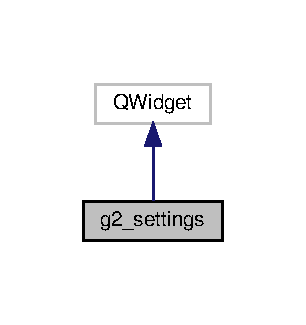
\includegraphics[width=147pt]{classg2__settings__inherit__graph}
\end{center}
\end{figure}


Collaboration diagram for g2\+\_\+settings\+:
\nopagebreak
\begin{figure}[H]
\begin{center}
\leavevmode
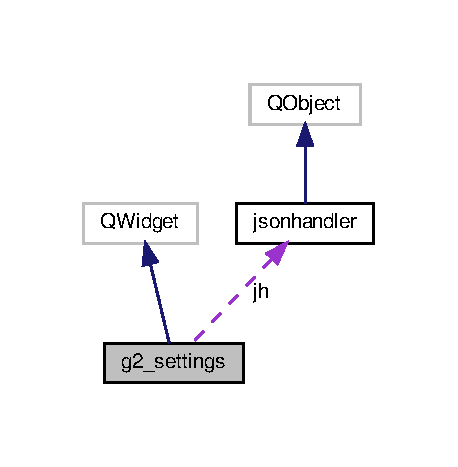
\includegraphics[width=220pt]{classg2__settings__coll__graph}
\end{center}
\end{figure}
\subsection*{Public Member Functions}
\begin{DoxyCompactItemize}
\item 
\hyperlink{classg2__settings_a3eb448dda234abb813d6a32bebebbcde}{g2\+\_\+settings} (Q\+Widget $\ast$parent=nullptr, Q\+Json\+Object json=\{\})
\begin{DoxyCompactList}\small\item\em \hyperlink{classg2__settings}{g2\+\_\+settings} constructor \end{DoxyCompactList}\item 
\mbox{\Hypertarget{classg2__settings_a597b2a521b8f9fae3d34dff56c196a7c}\label{classg2__settings_a597b2a521b8f9fae3d34dff56c196a7c}} 
void \hyperlink{classg2__settings_a597b2a521b8f9fae3d34dff56c196a7c}{set\+Grid\+Layout} ()
\begin{DoxyCompactList}\small\item\em set\+Grid\+Layout, sets the widgets of a grid layout \end{DoxyCompactList}\item 
\mbox{\Hypertarget{classg2__settings_a77c13b7cb2491bb0f68bb8a3ddf9de89}\label{classg2__settings_a77c13b7cb2491bb0f68bb8a3ddf9de89}} 
void \hyperlink{classg2__settings_a77c13b7cb2491bb0f68bb8a3ddf9de89}{create\+Difficulty\+Box} ()
\begin{DoxyCompactList}\small\item\em create\+Difficulty\+Box, creates the box of difficulty buttons \end{DoxyCompactList}\item 
\mbox{\Hypertarget{classg2__settings_a3c4aada8695c3d2b7d4869a4a5363863}\label{classg2__settings_a3c4aada8695c3d2b7d4869a4a5363863}} 
void \hyperlink{classg2__settings_a3c4aada8695c3d2b7d4869a4a5363863}{create\+Bg\+Box} ()
\begin{DoxyCompactList}\small\item\em create\+Bg\+Box, creates the box of bg buttons \end{DoxyCompactList}\end{DoxyCompactItemize}
\subsection*{Public Attributes}
\begin{DoxyCompactItemize}
\item 
\mbox{\Hypertarget{classg2__settings_aa2a37b0a03dd3615c8f1d66c71ee0100}\label{classg2__settings_aa2a37b0a03dd3615c8f1d66c71ee0100}} 
Q\+Push\+Button $\ast$ {\bfseries back\+Btn}
\item 
\mbox{\Hypertarget{classg2__settings_a58f30d865ee32cfb7d1a649caf997781}\label{classg2__settings_a58f30d865ee32cfb7d1a649caf997781}} 
Q\+Label $\ast$ {\bfseries title}
\item 
\mbox{\Hypertarget{classg2__settings_a4b3ad3277451f0e68b8ddf46f3a2c5dc}\label{classg2__settings_a4b3ad3277451f0e68b8ddf46f3a2c5dc}} 
Q\+Label $\ast$ {\bfseries diff\+Label}
\item 
\mbox{\Hypertarget{classg2__settings_aa72ff224374d24ff793bc30cabe5ee61}\label{classg2__settings_aa72ff224374d24ff793bc30cabe5ee61}} 
Q\+Label $\ast$ {\bfseries topic\+Label}
\item 
\mbox{\Hypertarget{classg2__settings_a6fec5a3eb1bb566ba438a4423968e202}\label{classg2__settings_a6fec5a3eb1bb566ba438a4423968e202}} 
Q\+Label $\ast$ {\bfseries bg\+Label}
\item 
\mbox{\Hypertarget{classg2__settings_a5f12d78e66315315bbb646c9ef3c2988}\label{classg2__settings_a5f12d78e66315315bbb646c9ef3c2988}} 
Q\+Push\+Button $\ast$ {\bfseries easy\+Btn}
\item 
\mbox{\Hypertarget{classg2__settings_aa3f14ee6604a3f234f5f406cf25bb4c9}\label{classg2__settings_aa3f14ee6604a3f234f5f406cf25bb4c9}} 
Q\+Push\+Button $\ast$ {\bfseries medium\+Btn}
\item 
\mbox{\Hypertarget{classg2__settings_a5577418d157d93609f9f9a51a5215373}\label{classg2__settings_a5577418d157d93609f9f9a51a5215373}} 
Q\+Push\+Button $\ast$ {\bfseries hard\+Btn}
\item 
\mbox{\Hypertarget{classg2__settings_a9d496428e50cf1a59abdb715666b3722}\label{classg2__settings_a9d496428e50cf1a59abdb715666b3722}} 
Q\+Group\+Box $\ast$ {\bfseries difficulty\+Box}
\item 
\mbox{\Hypertarget{classg2__settings_a10f8b06382d393ebdfc191311dc8d232}\label{classg2__settings_a10f8b06382d393ebdfc191311dc8d232}} 
Q\+H\+Box\+Layout $\ast$ {\bfseries diff\+Box\+Layout}
\item 
\mbox{\Hypertarget{classg2__settings_a8bb89596617af6af38e4e88f31f04a74}\label{classg2__settings_a8bb89596617af6af38e4e88f31f04a74}} 
Q\+Push\+Button $\ast$ {\bfseries bg1\+Btn}
\item 
\mbox{\Hypertarget{classg2__settings_a27baaf9a1bce1c7025358408979b74d2}\label{classg2__settings_a27baaf9a1bce1c7025358408979b74d2}} 
Q\+Push\+Button $\ast$ {\bfseries bg2\+Btn}
\item 
\mbox{\Hypertarget{classg2__settings_a46b7fa02e6e84f1b6d9f5bff74d0c8b2}\label{classg2__settings_a46b7fa02e6e84f1b6d9f5bff74d0c8b2}} 
Q\+Push\+Button $\ast$ {\bfseries bg3\+Btn}
\item 
\mbox{\Hypertarget{classg2__settings_a40794e8bcc953a858f2f5edc27271ee9}\label{classg2__settings_a40794e8bcc953a858f2f5edc27271ee9}} 
Q\+Group\+Box $\ast$ {\bfseries bg\+Box}
\item 
\mbox{\Hypertarget{classg2__settings_a8079d8ed4dffc37edc1bb1f003fda59a}\label{classg2__settings_a8079d8ed4dffc37edc1bb1f003fda59a}} 
Q\+H\+Box\+Layout $\ast$ {\bfseries bg\+Box\+Layout}
\item 
\mbox{\Hypertarget{classg2__settings_aa8b3e291021e81f7a90acab406b37546}\label{classg2__settings_aa8b3e291021e81f7a90acab406b37546}} 
Q\+Grid\+Layout $\ast$ {\bfseries grid}
\item 
\mbox{\Hypertarget{classg2__settings_a807af0ce75f72e99bb67a105dfa7ba41}\label{classg2__settings_a807af0ce75f72e99bb67a105dfa7ba41}} 
Q\+Json\+Object {\bfseries user\+Json}
\item 
\mbox{\Hypertarget{classg2__settings_a889d9695a4d3489fe256fe1ef00a9d17}\label{classg2__settings_a889d9695a4d3489fe256fe1ef00a9d17}} 
\hyperlink{classjsonhandler}{jsonhandler} $\ast$ {\bfseries jh} = new \hyperlink{classjsonhandler}{jsonhandler}()
\end{DoxyCompactItemize}


\subsection{Constructor \& Destructor Documentation}
\mbox{\Hypertarget{classg2__settings_a3eb448dda234abb813d6a32bebebbcde}\label{classg2__settings_a3eb448dda234abb813d6a32bebebbcde}} 
\index{g2\+\_\+settings@{g2\+\_\+settings}!g2\+\_\+settings@{g2\+\_\+settings}}
\index{g2\+\_\+settings@{g2\+\_\+settings}!g2\+\_\+settings@{g2\+\_\+settings}}
\subsubsection{\texorpdfstring{g2\+\_\+settings()}{g2\_settings()}}
{\footnotesize\ttfamily g2\+\_\+settings\+::g2\+\_\+settings (\begin{DoxyParamCaption}\item[{Q\+Widget $\ast$}]{parent = {\ttfamily nullptr},  }\item[{Q\+Json\+Object}]{json = {\ttfamily \{\}} }\end{DoxyParamCaption})\hspace{0.3cm}{\ttfamily [explicit]}}



\hyperlink{classg2__settings}{g2\+\_\+settings} constructor 


\begin{DoxyParams}{Parameters}
{\em parent,a} & nullptr to the Q\+Widget parent \\
\hline
{\em json,the} & Q\+Json\+Object for a given user. \\
\hline
\end{DoxyParams}


The documentation for this class was generated from the following files\+:\begin{DoxyCompactItemize}
\item 
\hyperlink{g2__settings_8h}{g2\+\_\+settings.\+h}\item 
\hyperlink{g2__settings_8cpp}{g2\+\_\+settings.\+cpp}\end{DoxyCompactItemize}

\hypertarget{classg2__setup}{}\section{g2\+\_\+setup Class Reference}
\label{classg2__setup}\index{g2\+\_\+setup@{g2\+\_\+setup}}


Inheritance diagram for g2\+\_\+setup\+:
\nopagebreak
\begin{figure}[H]
\begin{center}
\leavevmode
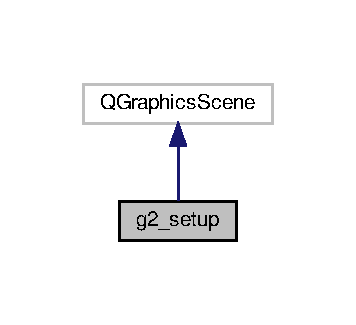
\includegraphics[width=171pt]{classg2__setup__inherit__graph}
\end{center}
\end{figure}


Collaboration diagram for g2\+\_\+setup\+:
\nopagebreak
\begin{figure}[H]
\begin{center}
\leavevmode
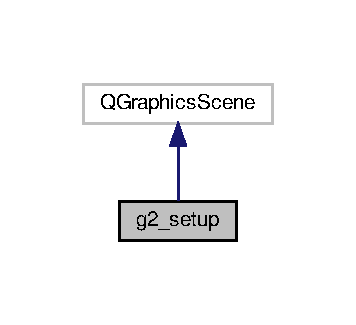
\includegraphics[width=171pt]{classg2__setup__coll__graph}
\end{center}
\end{figure}
\subsection*{Public Member Functions}
\begin{DoxyCompactItemize}
\item 
\hyperlink{classg2__setup_a1f4d4c1317565eb2bd9de3e2aa75f0a8}{g2\+\_\+setup} (Q\+Json\+Object json=\{\})
\begin{DoxyCompactList}\small\item\em \hyperlink{classg2__setup}{g2\+\_\+setup} constructor \end{DoxyCompactList}\end{DoxyCompactItemize}


\subsection{Constructor \& Destructor Documentation}
\mbox{\Hypertarget{classg2__setup_a1f4d4c1317565eb2bd9de3e2aa75f0a8}\label{classg2__setup_a1f4d4c1317565eb2bd9de3e2aa75f0a8}} 
\index{g2\+\_\+setup@{g2\+\_\+setup}!g2\+\_\+setup@{g2\+\_\+setup}}
\index{g2\+\_\+setup@{g2\+\_\+setup}!g2\+\_\+setup@{g2\+\_\+setup}}
\subsubsection{\texorpdfstring{g2\+\_\+setup()}{g2\_setup()}}
{\footnotesize\ttfamily g2\+\_\+setup\+::g2\+\_\+setup (\begin{DoxyParamCaption}\item[{Q\+Json\+Object}]{json = {\ttfamily \{\}} }\end{DoxyParamCaption})\hspace{0.3cm}{\ttfamily [explicit]}}



\hyperlink{classg2__setup}{g2\+\_\+setup} constructor 


\begin{DoxyParams}{Parameters}
{\em json,the} & player\textquotesingle{}s Q\+Json\+Object, initialized to an empty json object \\
\hline
\end{DoxyParams}


The documentation for this class was generated from the following files\+:\begin{DoxyCompactItemize}
\item 
g2\+\_\+setup.\+h\item 
g2\+\_\+setup.\+cpp\end{DoxyCompactItemize}

\hypertarget{classg2__startmenu}{}\section{g2\+\_\+startmenu Class Reference}
\label{classg2__startmenu}\index{g2\+\_\+startmenu@{g2\+\_\+startmenu}}


Inheritance diagram for g2\+\_\+startmenu\+:
\nopagebreak
\begin{figure}[H]
\begin{center}
\leavevmode
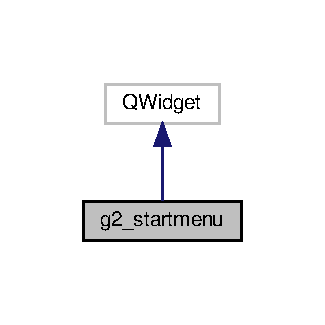
\includegraphics[width=156pt]{classg2__startmenu__inherit__graph}
\end{center}
\end{figure}


Collaboration diagram for g2\+\_\+startmenu\+:
\nopagebreak
\begin{figure}[H]
\begin{center}
\leavevmode
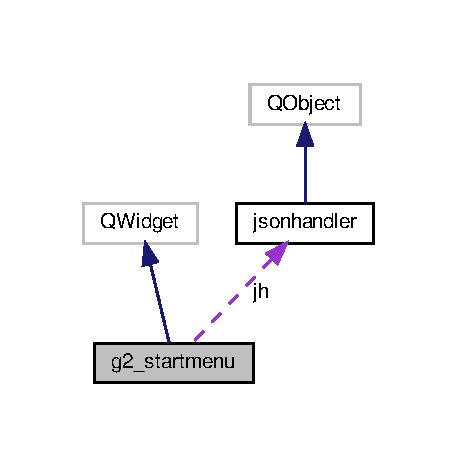
\includegraphics[width=220pt]{classg2__startmenu__coll__graph}
\end{center}
\end{figure}
\subsection*{Public Member Functions}
\begin{DoxyCompactItemize}
\item 
\hyperlink{classg2__startmenu_a64af506bcf731b441c756fdf389fdffe}{g2\+\_\+startmenu} (Q\+Widget $\ast$parent=nullptr, Q\+Json\+Object json=\{\})
\begin{DoxyCompactList}\small\item\em \hyperlink{classg2__startmenu}{g2\+\_\+startmenu} constructor \end{DoxyCompactList}\end{DoxyCompactItemize}
\subsection*{Public Attributes}
\begin{DoxyCompactItemize}
\item 
\mbox{\Hypertarget{classg2__startmenu_a01a68297e5716b4cf38a1f750afa8bcb}\label{classg2__startmenu_a01a68297e5716b4cf38a1f750afa8bcb}} 
Q\+Push\+Button $\ast$ {\bfseries play\+Btn}
\item 
\mbox{\Hypertarget{classg2__startmenu_a66ac1dda2bc33ef328b847d6125d7296}\label{classg2__startmenu_a66ac1dda2bc33ef328b847d6125d7296}} 
Q\+Push\+Button $\ast$ {\bfseries settings\+Btn}
\item 
\mbox{\Hypertarget{classg2__startmenu_a3cee06c0bc05368195dde924403951ac}\label{classg2__startmenu_a3cee06c0bc05368195dde924403951ac}} 
Q\+Push\+Button $\ast$ {\bfseries exit\+Btn}
\item 
\mbox{\Hypertarget{classg2__startmenu_a8944d2426bb7a093aafd1b47c40c3da8}\label{classg2__startmenu_a8944d2426bb7a093aafd1b47c40c3da8}} 
Q\+Label $\ast$ {\bfseries game\+Logo}
\item 
\mbox{\Hypertarget{classg2__startmenu_ad156cdc0c63d394dafa561c50d713f2c}\label{classg2__startmenu_ad156cdc0c63d394dafa561c50d713f2c}} 
Q\+V\+Box\+Layout $\ast$ {\bfseries v\+Layout}
\item 
\mbox{\Hypertarget{classg2__startmenu_ab0a28f0dc451be5b08b777aae37381eb}\label{classg2__startmenu_ab0a28f0dc451be5b08b777aae37381eb}} 
Q\+Json\+Object {\bfseries user\+Json}
\item 
\mbox{\Hypertarget{classg2__startmenu_a148870335d7c3196da239626772781d5}\label{classg2__startmenu_a148870335d7c3196da239626772781d5}} 
\hyperlink{classjsonhandler}{jsonhandler} $\ast$ {\bfseries jh} = new \hyperlink{classjsonhandler}{jsonhandler}()
\item 
\mbox{\Hypertarget{classg2__startmenu_a931b830df79ae145b5d8cf030357bc7b}\label{classg2__startmenu_a931b830df79ae145b5d8cf030357bc7b}} 
Q\+Graphics\+View $\ast$ {\bfseries v1}
\end{DoxyCompactItemize}


\subsection{Constructor \& Destructor Documentation}
\mbox{\Hypertarget{classg2__startmenu_a64af506bcf731b441c756fdf389fdffe}\label{classg2__startmenu_a64af506bcf731b441c756fdf389fdffe}} 
\index{g2\+\_\+startmenu@{g2\+\_\+startmenu}!g2\+\_\+startmenu@{g2\+\_\+startmenu}}
\index{g2\+\_\+startmenu@{g2\+\_\+startmenu}!g2\+\_\+startmenu@{g2\+\_\+startmenu}}
\subsubsection{\texorpdfstring{g2\+\_\+startmenu()}{g2\_startmenu()}}
{\footnotesize\ttfamily g2\+\_\+startmenu\+::g2\+\_\+startmenu (\begin{DoxyParamCaption}\item[{Q\+Widget $\ast$}]{parent = {\ttfamily nullptr},  }\item[{Q\+Json\+Object}]{json = {\ttfamily \{\}} }\end{DoxyParamCaption})\hspace{0.3cm}{\ttfamily [explicit]}}



\hyperlink{classg2__startmenu}{g2\+\_\+startmenu} constructor 


\begin{DoxyParams}{Parameters}
{\em parent,a} & pointer to a parent Q\+Widget, initialized to a nullptr \\
\hline
{\em json,the} & player\textquotesingle{}s Q\+Json\+Object, initialized to an empty json object \\
\hline
\end{DoxyParams}


The documentation for this class was generated from the following files\+:\begin{DoxyCompactItemize}
\item 
\hyperlink{g2__startmenu_8h}{g2\+\_\+startmenu.\+h}\item 
g2\+\_\+startmenu.\+cpp\end{DoxyCompactItemize}

\hypertarget{classgameLost}{}\section{game\+Lost Class Reference}
\label{classgameLost}\index{game\+Lost@{game\+Lost}}


Inheritance diagram for game\+Lost\+:
\nopagebreak
\begin{figure}[H]
\begin{center}
\leavevmode
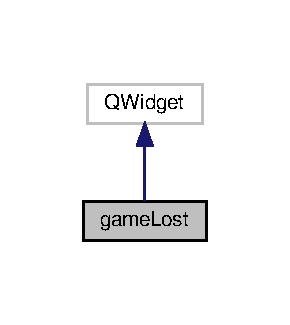
\includegraphics[width=139pt]{classgameLost__inherit__graph}
\end{center}
\end{figure}


Collaboration diagram for game\+Lost\+:
\nopagebreak
\begin{figure}[H]
\begin{center}
\leavevmode
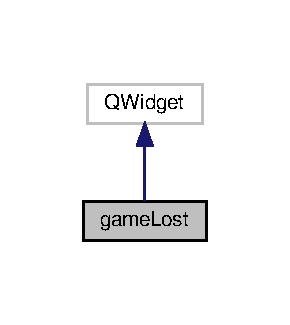
\includegraphics[width=139pt]{classgameLost__coll__graph}
\end{center}
\end{figure}
\subsection*{Public Member Functions}
\begin{DoxyCompactItemize}
\item 
\hyperlink{classgameLost_a845db0684130309120016d977920af72}{game\+Lost} (Q\+Widget $\ast$parent, Q\+Json\+Object json, int score\+Num, Q\+String game\+Id)
\begin{DoxyCompactList}\small\item\em \hyperlink{classgameLost}{game\+Lost} constructor \end{DoxyCompactList}\end{DoxyCompactItemize}


\subsection{Constructor \& Destructor Documentation}
\mbox{\Hypertarget{classgameLost_a845db0684130309120016d977920af72}\label{classgameLost_a845db0684130309120016d977920af72}} 
\index{game\+Lost@{game\+Lost}!game\+Lost@{game\+Lost}}
\index{game\+Lost@{game\+Lost}!game\+Lost@{game\+Lost}}
\subsubsection{\texorpdfstring{game\+Lost()}{gameLost()}}
{\footnotesize\ttfamily game\+Lost\+::game\+Lost (\begin{DoxyParamCaption}\item[{Q\+Widget $\ast$}]{parent,  }\item[{Q\+Json\+Object}]{json,  }\item[{int}]{score\+Num,  }\item[{Q\+String}]{game\+Id }\end{DoxyParamCaption})\hspace{0.3cm}{\ttfamily [explicit]}}



\hyperlink{classgameLost}{game\+Lost} constructor 


\begin{DoxyParams}{Parameters}
{\em parent,a} & pointer to a Q\+Widget parent \\
\hline
{\em json,a} & Q\+Json\+Object for a given user \\
\hline
{\em score\+Num,the} & player\textquotesingle{}s score. \\
\hline
{\em game\+Id,a} & Q\+String representing game Id. \char`\"{}game1\char`\"{} means Battleships and \char`\"{}game2\char`\"{} means Shooting Discs \\
\hline
\end{DoxyParams}


The documentation for this class was generated from the following files\+:\begin{DoxyCompactItemize}
\item 
gamelost.\+h\item 
gamelost.\+cpp\end{DoxyCompactItemize}

\hypertarget{classgameWon}{}\section{game\+Won Class Reference}
\label{classgameWon}\index{game\+Won@{game\+Won}}


Inheritance diagram for game\+Won\+:
\nopagebreak
\begin{figure}[H]
\begin{center}
\leavevmode
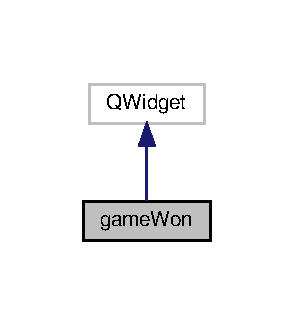
\includegraphics[width=141pt]{classgameWon__inherit__graph}
\end{center}
\end{figure}


Collaboration diagram for game\+Won\+:
\nopagebreak
\begin{figure}[H]
\begin{center}
\leavevmode
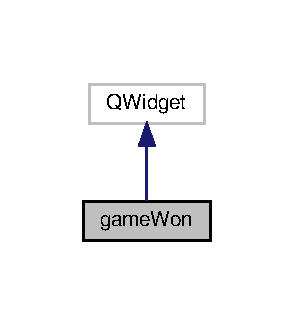
\includegraphics[width=141pt]{classgameWon__coll__graph}
\end{center}
\end{figure}
\subsection*{Public Member Functions}
\begin{DoxyCompactItemize}
\item 
\hyperlink{classgameWon_aa80eab42913e798314f5d3ab9305eeb8}{game\+Won} (Q\+Widget $\ast$parent, Q\+Json\+Object json, int score\+Num, Q\+String game\+Id)
\begin{DoxyCompactList}\small\item\em \hyperlink{classgameWon}{game\+Won} constructor \end{DoxyCompactList}\end{DoxyCompactItemize}


\subsection{Constructor \& Destructor Documentation}
\mbox{\Hypertarget{classgameWon_aa80eab42913e798314f5d3ab9305eeb8}\label{classgameWon_aa80eab42913e798314f5d3ab9305eeb8}} 
\index{game\+Won@{game\+Won}!game\+Won@{game\+Won}}
\index{game\+Won@{game\+Won}!game\+Won@{game\+Won}}
\subsubsection{\texorpdfstring{game\+Won()}{gameWon()}}
{\footnotesize\ttfamily game\+Won\+::game\+Won (\begin{DoxyParamCaption}\item[{Q\+Widget $\ast$}]{parent,  }\item[{Q\+Json\+Object}]{json,  }\item[{int}]{score\+Num,  }\item[{Q\+String}]{game\+Id }\end{DoxyParamCaption})\hspace{0.3cm}{\ttfamily [explicit]}}



\hyperlink{classgameWon}{game\+Won} constructor 


\begin{DoxyParams}{Parameters}
{\em parent,a} & pointer to a Q\+Widget parent \\
\hline
{\em json,a} & Q\+Json\+Object for a given user \\
\hline
{\em score\+Num,the} & player\textquotesingle{}s score. \\
\hline
{\em game\+Id,a} & Q\+String representing game Id. \char`\"{}game1\char`\"{} means Battleships and \char`\"{}game2\char`\"{} means Shooting Discs \\
\hline
\end{DoxyParams}


The documentation for this class was generated from the following files\+:\begin{DoxyCompactItemize}
\item 
gamewon.\+h\item 
gamewon.\+cpp\end{DoxyCompactItemize}

\hypertarget{classjsonhandler}{}\section{jsonhandler Class Reference}
\label{classjsonhandler}\index{jsonhandler@{jsonhandler}}


Inheritance diagram for jsonhandler\+:
\nopagebreak
\begin{figure}[H]
\begin{center}
\leavevmode
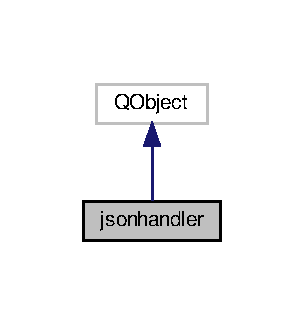
\includegraphics[width=146pt]{classjsonhandler__inherit__graph}
\end{center}
\end{figure}


Collaboration diagram for jsonhandler\+:
\nopagebreak
\begin{figure}[H]
\begin{center}
\leavevmode
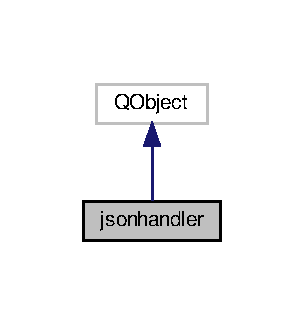
\includegraphics[width=146pt]{classjsonhandler__coll__graph}
\end{center}
\end{figure}
\subsection*{Public Member Functions}
\begin{DoxyCompactItemize}
\item 
\hyperlink{classjsonhandler_ac54df4dbf7d14ad39c30d3b7efa8876d}{jsonhandler} (Q\+Object $\ast$parent=nullptr)
\begin{DoxyCompactList}\small\item\em jsonhandler constructor \end{DoxyCompactList}\item 
Q\+Json\+Array \hyperlink{classjsonhandler_aebc2c7497f32984133a9352d03fd06e7}{read\+File} (Q\+String path)
\begin{DoxyCompactList}\small\item\em a function that opens a file, reads it, and stores its data in a Q\+J\+Son\+Array \end{DoxyCompactList}\item 
void \hyperlink{classjsonhandler_a1439109eb8fa7fffde057548afd8e3bb}{write\+File} (Q\+String path)
\begin{DoxyCompactList}\small\item\em a function that writes to a file \end{DoxyCompactList}\item 
void \hyperlink{classjsonhandler_a254e472bc7f40602a5287015591309af}{update\+Userarr} (Q\+Json\+Object userjson)
\begin{DoxyCompactList}\small\item\em a function that updates a user Q\+Json\+Object in jsonhandler\+::userarr \end{DoxyCompactList}\item 
Q\+Json\+Object \hyperlink{classjsonhandler_a9bb2dc65754d170a493d60e82cc5ff18}{update\+Bonus} (Q\+Json\+Object userjson, int bonus)
\begin{DoxyCompactList}\small\item\em update\+Bonus, updates the bonus points of a user in game 2 \end{DoxyCompactList}\item 
Q\+Json\+Object \hyperlink{classjsonhandler_a80a0d472fc04d855cc91c3a39185d344}{check\+User} (Q\+String username, Q\+String password)
\begin{DoxyCompactList}\small\item\em a function that checks whether the username and password match the credentials of the registered user \end{DoxyCompactList}\item 
bool \hyperlink{classjsonhandler_a3860da83ed54e86300f756f5b66c3d68}{check\+User} (Q\+String username)
\begin{DoxyCompactList}\small\item\em Overloaded check\+User function that checks if the username is taken or not. \end{DoxyCompactList}\item 
void \hyperlink{classjsonhandler_a93f4319d533f65208a05f572b4fd1f76}{insert\+User} (Q\+Json\+Object userjson)
\begin{DoxyCompactList}\small\item\em a function that inserts a new user Q\+Json\+Object in jsonhandler\+::userarr and writes the updated array to data.\+json \end{DoxyCompactList}\item 
int \hyperlink{classjsonhandler_ad1a3458ade52adb1e44fdf147450f60b}{get\+Highscore} (Q\+Json\+Object userjson, Q\+String game\+Id)
\begin{DoxyCompactList}\small\item\em gets the highscore of a user in either Battleships or Shooting Discs. \end{DoxyCompactList}\item 
Q\+Json\+Array \hyperlink{classjsonhandler_aba9044f8e89f6bbe9a136d27062b7358}{get\+Scores\+Arr} (Q\+Json\+Object userjson, Q\+String game\+Id)
\begin{DoxyCompactList}\small\item\em gets the scores arry of a user in either Battleships or Shooting Discs. \end{DoxyCompactList}\item 
Q\+Json\+Object \hyperlink{classjsonhandler_a383b010b1318971dc8170d2744f25342}{update\+Scores} (Q\+Json\+Object userjson, int new\+Score, Q\+String game\+Id)
\begin{DoxyCompactList}\small\item\em adds the new score to the user\textquotesingle{}s scores array in either Battleships or Shooting Discs. \end{DoxyCompactList}\item 
Q\+Json\+Object \hyperlink{classjsonhandler_ab702fe91f4f95c309d7fed4402b05dcc}{get\+Global\+H\+S\+And\+Rank} (int hs, Q\+String game\+ID)
\begin{DoxyCompactList}\small\item\em retrieves the global highscore of a game and computes the rank of the player \end{DoxyCompactList}\item 
Q\+String \hyperlink{classjsonhandler_a3ebc5fcd86eeda6e9b54410986d268fc}{get\+Bg\+Color} (Q\+Json\+Object userjson, Q\+String game\+ID)
\begin{DoxyCompactList}\small\item\em gets the background color as specified in the game settings in a user\textquotesingle{}s Q\+Json\+Object \end{DoxyCompactList}\item 
Q\+String \hyperlink{classjsonhandler_ad23eb6976b88403ec2b91f62cff8b0d0}{get\+Bg\+Img} (Q\+Json\+Object userjson, Q\+String game\+ID)
\begin{DoxyCompactList}\small\item\em get\+Bg\+Img, retrieves the path to the background image in userjson \end{DoxyCompactList}\end{DoxyCompactItemize}
\subsection*{Public Attributes}
\begin{DoxyCompactItemize}
\item 
\mbox{\Hypertarget{classjsonhandler_a9c1236ad63624244d0775d1abec70c7c}\label{classjsonhandler_a9c1236ad63624244d0775d1abec70c7c}} 
Q\+String {\bfseries user\+Path} = \char`\"{}../repos/lama\+\_\+milia\+\_\+rana/project\+\_\+/data.\+json\char`\"{}
\item 
\mbox{\Hypertarget{classjsonhandler_a8f8b279a35cdd398e62dc160b706dcdd}\label{classjsonhandler_a8f8b279a35cdd398e62dc160b706dcdd}} 
Q\+String {\bfseries quests\+Path} = \char`\"{}../repos/lama\+\_\+milia\+\_\+rana/project\+\_\+/questions.\+json\char`\"{}
\item 
\mbox{\Hypertarget{classjsonhandler_a4571bd5c720772f91bcfa6cfbcc0ecfb}\label{classjsonhandler_a4571bd5c720772f91bcfa6cfbcc0ecfb}} 
Q\+Json\+Array {\bfseries userarr}
\end{DoxyCompactItemize}


\subsection{Constructor \& Destructor Documentation}
\mbox{\Hypertarget{classjsonhandler_ac54df4dbf7d14ad39c30d3b7efa8876d}\label{classjsonhandler_ac54df4dbf7d14ad39c30d3b7efa8876d}} 
\index{jsonhandler@{jsonhandler}!jsonhandler@{jsonhandler}}
\index{jsonhandler@{jsonhandler}!jsonhandler@{jsonhandler}}
\subsubsection{\texorpdfstring{jsonhandler()}{jsonhandler()}}
{\footnotesize\ttfamily jsonhandler\+::jsonhandler (\begin{DoxyParamCaption}\item[{Q\+Object $\ast$}]{parent = {\ttfamily nullptr} }\end{DoxyParamCaption})\hspace{0.3cm}{\ttfamily [explicit]}}



jsonhandler constructor 


\begin{DoxyParams}{Parameters}
{\em parent,a} & pointer to a Q\+Object, initally a nullptr.\\
\hline
\end{DoxyParams}
The constructor creates an instance of jsonhandler class and calls the readfile function with user\+Path passed as an argument. The result of read\+File is stored in userarr 

\subsection{Member Function Documentation}
\mbox{\Hypertarget{classjsonhandler_a80a0d472fc04d855cc91c3a39185d344}\label{classjsonhandler_a80a0d472fc04d855cc91c3a39185d344}} 
\index{jsonhandler@{jsonhandler}!check\+User@{check\+User}}
\index{check\+User@{check\+User}!jsonhandler@{jsonhandler}}
\subsubsection{\texorpdfstring{check\+User()}{checkUser()}\hspace{0.1cm}{\footnotesize\ttfamily [1/2]}}
{\footnotesize\ttfamily Q\+Json\+Object jsonhandler\+::check\+User (\begin{DoxyParamCaption}\item[{Q\+String}]{username,  }\item[{Q\+String}]{password }\end{DoxyParamCaption})}



a function that checks whether the username and password match the credentials of the registered user 


\begin{DoxyParams}{Parameters}
{\em username} & (Q\+String). \\
\hline
{\em password} & (Q\+String). \\
\hline
\end{DoxyParams}
\begin{DoxyReturn}{Returns}
Q\+Json\+Object containing the user with matching username and password. Returns an empty object otherwise. 
\end{DoxyReturn}
\mbox{\Hypertarget{classjsonhandler_a3860da83ed54e86300f756f5b66c3d68}\label{classjsonhandler_a3860da83ed54e86300f756f5b66c3d68}} 
\index{jsonhandler@{jsonhandler}!check\+User@{check\+User}}
\index{check\+User@{check\+User}!jsonhandler@{jsonhandler}}
\subsubsection{\texorpdfstring{check\+User()}{checkUser()}\hspace{0.1cm}{\footnotesize\ttfamily [2/2]}}
{\footnotesize\ttfamily bool jsonhandler\+::check\+User (\begin{DoxyParamCaption}\item[{Q\+String}]{username }\end{DoxyParamCaption})}



Overloaded check\+User function that checks if the username is taken or not. 


\begin{DoxyParams}{Parameters}
{\em username} & (Qstring) \\
\hline
\end{DoxyParams}
\begin{DoxyReturn}{Returns}
bool, true in case the user is taken, false otherwise. 
\end{DoxyReturn}
\mbox{\Hypertarget{classjsonhandler_a3ebc5fcd86eeda6e9b54410986d268fc}\label{classjsonhandler_a3ebc5fcd86eeda6e9b54410986d268fc}} 
\index{jsonhandler@{jsonhandler}!get\+Bg\+Color@{get\+Bg\+Color}}
\index{get\+Bg\+Color@{get\+Bg\+Color}!jsonhandler@{jsonhandler}}
\subsubsection{\texorpdfstring{get\+Bg\+Color()}{getBgColor()}}
{\footnotesize\ttfamily Q\+String jsonhandler\+::get\+Bg\+Color (\begin{DoxyParamCaption}\item[{Q\+Json\+Object}]{userjson,  }\item[{Q\+String}]{game\+Id }\end{DoxyParamCaption})}



gets the background color as specified in the game settings in a user\textquotesingle{}s Q\+Json\+Object 


\begin{DoxyParams}{Parameters}
{\em userjson,a} & Q\+Json\+Object of a given user \\
\hline
{\em game\+ID,the} & ID of the game \\
\hline
\end{DoxyParams}
\begin{DoxyReturn}{Returns}
Q\+String containing the bg color in the following format \textquotesingle{}\#hexrepresentation\textquotesingle{} 
\end{DoxyReturn}
\mbox{\Hypertarget{classjsonhandler_ad23eb6976b88403ec2b91f62cff8b0d0}\label{classjsonhandler_ad23eb6976b88403ec2b91f62cff8b0d0}} 
\index{jsonhandler@{jsonhandler}!get\+Bg\+Img@{get\+Bg\+Img}}
\index{get\+Bg\+Img@{get\+Bg\+Img}!jsonhandler@{jsonhandler}}
\subsubsection{\texorpdfstring{get\+Bg\+Img()}{getBgImg()}}
{\footnotesize\ttfamily Q\+String jsonhandler\+::get\+Bg\+Img (\begin{DoxyParamCaption}\item[{Q\+Json\+Object}]{userjson,  }\item[{Q\+String}]{game\+Id }\end{DoxyParamCaption})}



get\+Bg\+Img, retrieves the path to the background image in userjson 


\begin{DoxyParams}{Parameters}
{\em userjson} & \\
\hline
{\em game\+ID} & \\
\hline
\end{DoxyParams}
\begin{DoxyReturn}{Returns}
the path to the bg img 
\end{DoxyReturn}
\mbox{\Hypertarget{classjsonhandler_ab702fe91f4f95c309d7fed4402b05dcc}\label{classjsonhandler_ab702fe91f4f95c309d7fed4402b05dcc}} 
\index{jsonhandler@{jsonhandler}!get\+Global\+H\+S\+And\+Rank@{get\+Global\+H\+S\+And\+Rank}}
\index{get\+Global\+H\+S\+And\+Rank@{get\+Global\+H\+S\+And\+Rank}!jsonhandler@{jsonhandler}}
\subsubsection{\texorpdfstring{get\+Global\+H\+S\+And\+Rank()}{getGlobalHSAndRank()}}
{\footnotesize\ttfamily Q\+Json\+Object jsonhandler\+::get\+Global\+H\+S\+And\+Rank (\begin{DoxyParamCaption}\item[{int}]{hs,  }\item[{Q\+String}]{game\+ID }\end{DoxyParamCaption})}



retrieves the global highscore of a game and computes the rank of the player 


\begin{DoxyParams}{Parameters}
{\em hs,int,the} & highscore of the player. \\
\hline
{\em game\+ID,the} & ID of the game \\
\hline
\end{DoxyParams}
\begin{DoxyReturn}{Returns}
Q\+Json\+Object containing the global highscore and player rank. 
\end{DoxyReturn}
\mbox{\Hypertarget{classjsonhandler_ad1a3458ade52adb1e44fdf147450f60b}\label{classjsonhandler_ad1a3458ade52adb1e44fdf147450f60b}} 
\index{jsonhandler@{jsonhandler}!get\+Highscore@{get\+Highscore}}
\index{get\+Highscore@{get\+Highscore}!jsonhandler@{jsonhandler}}
\subsubsection{\texorpdfstring{get\+Highscore()}{getHighscore()}}
{\footnotesize\ttfamily int jsonhandler\+::get\+Highscore (\begin{DoxyParamCaption}\item[{Q\+Json\+Object}]{userjson,  }\item[{Q\+String}]{game\+Id }\end{DoxyParamCaption})}



gets the highscore of a user in either Battleships or Shooting Discs. 


\begin{DoxyParams}{Parameters}
{\em userjson,a} & Q\+Json\+Object of a given user. \\
\hline
{\em game\+Id,a} & Q\+String containing game ID. \\
\hline
\end{DoxyParams}
\begin{DoxyReturn}{Returns}
int, the highscore 
\end{DoxyReturn}
\mbox{\Hypertarget{classjsonhandler_aba9044f8e89f6bbe9a136d27062b7358}\label{classjsonhandler_aba9044f8e89f6bbe9a136d27062b7358}} 
\index{jsonhandler@{jsonhandler}!get\+Scores\+Arr@{get\+Scores\+Arr}}
\index{get\+Scores\+Arr@{get\+Scores\+Arr}!jsonhandler@{jsonhandler}}
\subsubsection{\texorpdfstring{get\+Scores\+Arr()}{getScoresArr()}}
{\footnotesize\ttfamily Q\+Json\+Array jsonhandler\+::get\+Scores\+Arr (\begin{DoxyParamCaption}\item[{Q\+Json\+Object}]{userjson,  }\item[{Q\+String}]{game\+Id }\end{DoxyParamCaption})}



gets the scores arry of a user in either Battleships or Shooting Discs. 


\begin{DoxyParams}{Parameters}
{\em userjson,a} & Q\+Json\+Object of a given user. \\
\hline
{\em game\+Id,a} & Q\+String containing game ID. \\
\hline
\end{DoxyParams}
\begin{DoxyReturn}{Returns}
Q\+Json\+Array, the scores array 
\end{DoxyReturn}
\mbox{\Hypertarget{classjsonhandler_a93f4319d533f65208a05f572b4fd1f76}\label{classjsonhandler_a93f4319d533f65208a05f572b4fd1f76}} 
\index{jsonhandler@{jsonhandler}!insert\+User@{insert\+User}}
\index{insert\+User@{insert\+User}!jsonhandler@{jsonhandler}}
\subsubsection{\texorpdfstring{insert\+User()}{insertUser()}}
{\footnotesize\ttfamily void jsonhandler\+::insert\+User (\begin{DoxyParamCaption}\item[{Q\+Json\+Object}]{userjson }\end{DoxyParamCaption})}



a function that inserts a new user Q\+Json\+Object in jsonhandler\+::userarr and writes the updated array to data.\+json 


\begin{DoxyParams}{Parameters}
{\em userjson,the} & new Q\+Json\+Object to be added. \\
\hline
\end{DoxyParams}
\mbox{\Hypertarget{classjsonhandler_aebc2c7497f32984133a9352d03fd06e7}\label{classjsonhandler_aebc2c7497f32984133a9352d03fd06e7}} 
\index{jsonhandler@{jsonhandler}!read\+File@{read\+File}}
\index{read\+File@{read\+File}!jsonhandler@{jsonhandler}}
\subsubsection{\texorpdfstring{read\+File()}{readFile()}}
{\footnotesize\ttfamily Q\+Json\+Array jsonhandler\+::read\+File (\begin{DoxyParamCaption}\item[{Q\+String}]{path }\end{DoxyParamCaption})}



a function that opens a file, reads it, and stores its data in a Q\+J\+Son\+Array 


\begin{DoxyParams}{Parameters}
{\em path,a} & Q\+String containing the path to the json file. \\
\hline
\end{DoxyParams}
\begin{DoxyReturn}{Returns}
Q\+Json\+Array containing the result of read\+File. 
\end{DoxyReturn}
\mbox{\Hypertarget{classjsonhandler_a9bb2dc65754d170a493d60e82cc5ff18}\label{classjsonhandler_a9bb2dc65754d170a493d60e82cc5ff18}} 
\index{jsonhandler@{jsonhandler}!update\+Bonus@{update\+Bonus}}
\index{update\+Bonus@{update\+Bonus}!jsonhandler@{jsonhandler}}
\subsubsection{\texorpdfstring{update\+Bonus()}{updateBonus()}}
{\footnotesize\ttfamily Q\+Json\+Object jsonhandler\+::update\+Bonus (\begin{DoxyParamCaption}\item[{Q\+Json\+Object}]{userjson,  }\item[{int}]{bonus }\end{DoxyParamCaption})}



update\+Bonus, updates the bonus points of a user in game 2 


\begin{DoxyParams}{Parameters}
{\em userjson} & \\
\hline
{\em bonus} & \\
\hline
\end{DoxyParams}
\begin{DoxyReturn}{Returns}
the new updated json object 
\end{DoxyReturn}
\mbox{\Hypertarget{classjsonhandler_a383b010b1318971dc8170d2744f25342}\label{classjsonhandler_a383b010b1318971dc8170d2744f25342}} 
\index{jsonhandler@{jsonhandler}!update\+Scores@{update\+Scores}}
\index{update\+Scores@{update\+Scores}!jsonhandler@{jsonhandler}}
\subsubsection{\texorpdfstring{update\+Scores()}{updateScores()}}
{\footnotesize\ttfamily Q\+Json\+Object jsonhandler\+::update\+Scores (\begin{DoxyParamCaption}\item[{Q\+Json\+Object}]{userjson,  }\item[{int}]{new\+Score,  }\item[{Q\+String}]{game\+Id }\end{DoxyParamCaption})}



adds the new score to the user\textquotesingle{}s scores array in either Battleships or Shooting Discs. 


\begin{DoxyParams}{Parameters}
{\em userjson,a} & Q\+Json\+Object of a given user. \\
\hline
{\em new\+Score,int,the} & new score. \\
\hline
{\em game\+Id,a} & Q\+String containing game ID. \\
\hline
\end{DoxyParams}
\begin{DoxyReturn}{Returns}
Q\+Json\+Array, the updated scores array 
\end{DoxyReturn}
\mbox{\Hypertarget{classjsonhandler_a254e472bc7f40602a5287015591309af}\label{classjsonhandler_a254e472bc7f40602a5287015591309af}} 
\index{jsonhandler@{jsonhandler}!update\+Userarr@{update\+Userarr}}
\index{update\+Userarr@{update\+Userarr}!jsonhandler@{jsonhandler}}
\subsubsection{\texorpdfstring{update\+Userarr()}{updateUserarr()}}
{\footnotesize\ttfamily void jsonhandler\+::update\+Userarr (\begin{DoxyParamCaption}\item[{Q\+Json\+Object}]{userjson }\end{DoxyParamCaption})}



a function that updates a user Q\+Json\+Object in jsonhandler\+::userarr 


\begin{DoxyParams}{Parameters}
{\em userjson,the} & Q\+Json\+Object to be updated. \\
\hline
\end{DoxyParams}
\mbox{\Hypertarget{classjsonhandler_a1439109eb8fa7fffde057548afd8e3bb}\label{classjsonhandler_a1439109eb8fa7fffde057548afd8e3bb}} 
\index{jsonhandler@{jsonhandler}!write\+File@{write\+File}}
\index{write\+File@{write\+File}!jsonhandler@{jsonhandler}}
\subsubsection{\texorpdfstring{write\+File()}{writeFile()}}
{\footnotesize\ttfamily void jsonhandler\+::write\+File (\begin{DoxyParamCaption}\item[{Q\+String}]{path }\end{DoxyParamCaption})}



a function that writes to a file 


\begin{DoxyParams}{Parameters}
{\em path,a} & Q\+String containing the path to the json file. \\
\hline
\end{DoxyParams}


The documentation for this class was generated from the following files\+:\begin{DoxyCompactItemize}
\item 
\hyperlink{jsonhandler_8h}{jsonhandler.\+h}\item 
\hyperlink{jsonhandler_8cpp}{jsonhandler.\+cpp}\end{DoxyCompactItemize}

\hypertarget{classmain}{}\section{main Class Reference}
\label{classmain}\index{main@{main}}


The documentation for this class was generated from the following file\+:\begin{DoxyCompactItemize}
\item 
main.\+h\end{DoxyCompactItemize}

\hypertarget{classnoTurns}{}\section{no\+Turns Class Reference}
\label{classnoTurns}\index{no\+Turns@{no\+Turns}}


Inheritance diagram for no\+Turns\+:
\nopagebreak
\begin{figure}[H]
\begin{center}
\leavevmode
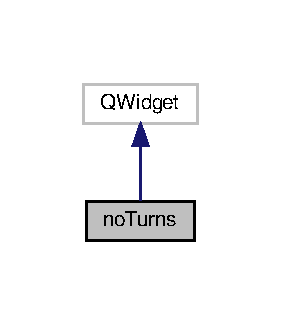
\includegraphics[width=135pt]{classnoTurns__inherit__graph}
\end{center}
\end{figure}


Collaboration diagram for no\+Turns\+:
\nopagebreak
\begin{figure}[H]
\begin{center}
\leavevmode
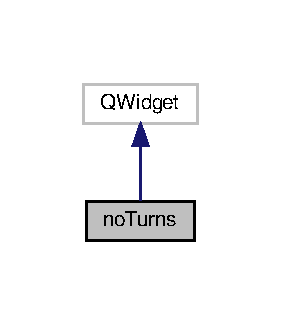
\includegraphics[width=135pt]{classnoTurns__coll__graph}
\end{center}
\end{figure}
\subsection*{Public Member Functions}
\begin{DoxyCompactItemize}
\item 
\hyperlink{classnoTurns_a602def6b039215fd6035a4b8d349b571}{no\+Turns} (Q\+Widget $\ast$parent, Q\+Json\+Object json, int score\+Num)
\begin{DoxyCompactList}\small\item\em \hyperlink{classnoTurns}{no\+Turns} constructor \end{DoxyCompactList}\end{DoxyCompactItemize}


\subsection{Constructor \& Destructor Documentation}
\mbox{\Hypertarget{classnoTurns_a602def6b039215fd6035a4b8d349b571}\label{classnoTurns_a602def6b039215fd6035a4b8d349b571}} 
\index{no\+Turns@{no\+Turns}!no\+Turns@{no\+Turns}}
\index{no\+Turns@{no\+Turns}!no\+Turns@{no\+Turns}}
\subsubsection{\texorpdfstring{no\+Turns()}{noTurns()}}
{\footnotesize\ttfamily no\+Turns\+::no\+Turns (\begin{DoxyParamCaption}\item[{Q\+Widget $\ast$}]{parent,  }\item[{Q\+Json\+Object}]{json,  }\item[{int}]{score\+Num }\end{DoxyParamCaption})\hspace{0.3cm}{\ttfamily [explicit]}}



\hyperlink{classnoTurns}{no\+Turns} constructor 


\begin{DoxyParams}{Parameters}
{\em parent,a} & pointer to a Q\+Widget parent \\
\hline
{\em json,a} & Q\+Json\+Object for a given user \\
\hline
{\em score\+Num,the} & player\textquotesingle{}s score. \\
\hline
\end{DoxyParams}


The documentation for this class was generated from the following files\+:\begin{DoxyCompactItemize}
\item 
noturns.\+h\item 
noturns.\+cpp\end{DoxyCompactItemize}

\hypertarget{classplayasguest}{}\section{playasguest Class Reference}
\label{classplayasguest}\index{playasguest@{playasguest}}


Inheritance diagram for playasguest\+:
\nopagebreak
\begin{figure}[H]
\begin{center}
\leavevmode
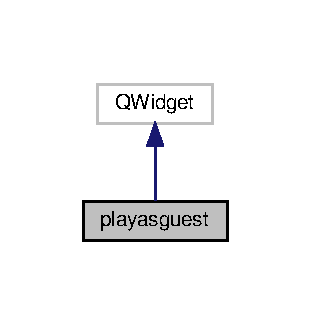
\includegraphics[width=149pt]{classplayasguest__inherit__graph}
\end{center}
\end{figure}


Collaboration diagram for playasguest\+:
\nopagebreak
\begin{figure}[H]
\begin{center}
\leavevmode
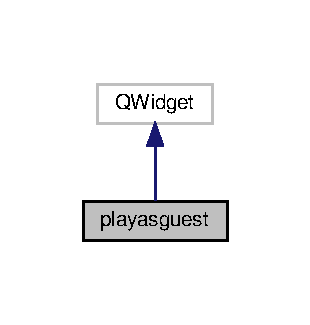
\includegraphics[width=149pt]{classplayasguest__coll__graph}
\end{center}
\end{figure}
\subsection*{Public Member Functions}
\begin{DoxyCompactItemize}
\item 
\hyperlink{classplayasguest_ad5c1931e8115567e7f11452e88b73d06}{playasguest} (Q\+Widget $\ast$parent=nullptr)
\begin{DoxyCompactList}\small\item\em playasguest constructor \end{DoxyCompactList}\end{DoxyCompactItemize}


\subsection{Constructor \& Destructor Documentation}
\mbox{\Hypertarget{classplayasguest_ad5c1931e8115567e7f11452e88b73d06}\label{classplayasguest_ad5c1931e8115567e7f11452e88b73d06}} 
\index{playasguest@{playasguest}!playasguest@{playasguest}}
\index{playasguest@{playasguest}!playasguest@{playasguest}}
\subsubsection{\texorpdfstring{playasguest()}{playasguest()}}
{\footnotesize\ttfamily playasguest\+::playasguest (\begin{DoxyParamCaption}\item[{Q\+Widget $\ast$}]{parent = {\ttfamily nullptr} }\end{DoxyParamCaption})\hspace{0.3cm}{\ttfamily [explicit]}}



playasguest constructor 


\begin{DoxyParams}{Parameters}
{\em parent,a} & pointer to the parent widget \\
\hline
\end{DoxyParams}


The documentation for this class was generated from the following files\+:\begin{DoxyCompactItemize}
\item 
playasguest.\+h\item 
playasguest.\+cpp\end{DoxyCompactItemize}

\hypertarget{classquests}{}\section{quests Class Reference}
\label{classquests}\index{quests@{quests}}


Inheritance diagram for quests\+:
\nopagebreak
\begin{figure}[H]
\begin{center}
\leavevmode
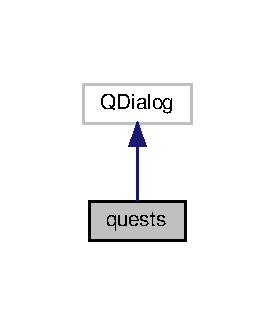
\includegraphics[width=132pt]{classquests__inherit__graph}
\end{center}
\end{figure}


Collaboration diagram for quests\+:
\nopagebreak
\begin{figure}[H]
\begin{center}
\leavevmode
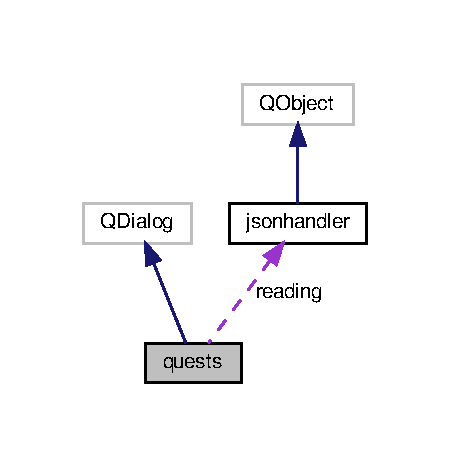
\includegraphics[width=216pt]{classquests__coll__graph}
\end{center}
\end{figure}
\subsection*{Public Slots}
\begin{DoxyCompactItemize}
\item 
\mbox{\Hypertarget{classquests_a2fd07763aff26aae5036acb169719fff}\label{classquests_a2fd07763aff26aae5036acb169719fff}} 
void \hyperlink{classquests_a2fd07763aff26aae5036acb169719fff}{checkanswer1} ()
\begin{DoxyCompactList}\small\item\em checks whether the chosen pushbutton contains the correct answer. The function displays wrng Q\+Message\+Box in case the answer is incorrect and right Q\+Message\+Box otherwise. \end{DoxyCompactList}\item 
\mbox{\Hypertarget{classquests_aff4a72bbc6183f358be72359f576ffed}\label{classquests_aff4a72bbc6183f358be72359f576ffed}} 
void \hyperlink{classquests_aff4a72bbc6183f358be72359f576ffed}{checkanswer2} ()
\begin{DoxyCompactList}\small\item\em checks whether the chosen pushbutton contains the correct answer. The function displays wrng Q\+Message\+Box in case the answer is incorrect and right Q\+Message\+Box otherwise. \end{DoxyCompactList}\item 
\mbox{\Hypertarget{classquests_aa40aba6d49a76ce0f3110046b0c0f72e}\label{classquests_aa40aba6d49a76ce0f3110046b0c0f72e}} 
void \hyperlink{classquests_aa40aba6d49a76ce0f3110046b0c0f72e}{checkanswer3} ()
\begin{DoxyCompactList}\small\item\em checks whether the chosen pushbutton contains the correct answer. The function displays wrng Q\+Message\+Box in case the answer is incorrect and right Q\+Message\+Box otherwise. \end{DoxyCompactList}\item 
\mbox{\Hypertarget{classquests_a4b75d0858f37450128457d565afe4411}\label{classquests_a4b75d0858f37450128457d565afe4411}} 
void \hyperlink{classquests_a4b75d0858f37450128457d565afe4411}{checkanswer4} ()
\begin{DoxyCompactList}\small\item\em checks whether the chosen pushbutton contains the correct answer. The function displays wrng Q\+Message\+Box in case the answer is incorrect and right Q\+Message\+Box otherwise. \end{DoxyCompactList}\end{DoxyCompactItemize}
\subsection*{Public Member Functions}
\begin{DoxyCompactItemize}
\item 
\hyperlink{classquests_a54541119f891382cdda66b247edc090b}{quests} (Q\+Widget $\ast$parent=nullptr, Q\+Json\+Object json=\{\}, int count=0)
\begin{DoxyCompactList}\small\item\em quests constructor \end{DoxyCompactList}\item 
\mbox{\Hypertarget{classquests_a3b538c389f15ef6f79fdcdf114b27392}\label{classquests_a3b538c389f15ef6f79fdcdf114b27392}} 
void \hyperlink{classquests_a3b538c389f15ef6f79fdcdf114b27392}{create\+Ans\+Box} ()
\begin{DoxyCompactList}\small\item\em sets the widget of the answers layout \end{DoxyCompactList}\item 
\mbox{\Hypertarget{classquests_aca51e37f6ef603d3caaff95661eed638}\label{classquests_aca51e37f6ef603d3caaff95661eed638}} 
void \hyperlink{classquests_aca51e37f6ef603d3caaff95661eed638}{set\+Grid\+Layout} ()
\begin{DoxyCompactList}\small\item\em sets the widgets of the grid layout \end{DoxyCompactList}\item 
Q\+String \hyperlink{classquests_a99d693e004d57fbea81a6ef92d843e32}{mapdiff} (int d)
\begin{DoxyCompactList}\small\item\em maps an integer to the corresponding difficulty \end{DoxyCompactList}\item 
Q\+String \hyperlink{classquests_a360c52960fcebef73ffd987d5fe0cefc}{maptop} (int t)
\begin{DoxyCompactList}\small\item\em maps an integer to the corresponding topic \end{DoxyCompactList}\item 
Q\+Json\+Array \hyperlink{classquests_a1c75a4a0a1e429e5ed5b0a7c08a842cf}{getquest} (Q\+String d, Q\+String t)
\begin{DoxyCompactList}\small\item\em Retrieves array of questions of a difficulty d and topic t. \end{DoxyCompactList}\item 
void \hyperlink{classquests_a63b57d7fc7d4aa382da23d9a4592545e}{setquests} (Q\+Json\+Object quest)
\begin{DoxyCompactList}\small\item\em Sets the question in the Q\+Dialog. \end{DoxyCompactList}\item 
\mbox{\Hypertarget{classquests_a16ce1db433118576119829773238ce9d}\label{classquests_a16ce1db433118576119829773238ce9d}} 
void \hyperlink{classquests_a16ce1db433118576119829773238ce9d}{init\+Bg} ()
\begin{DoxyCompactList}\small\item\em initializes the background color of the Q\+Widget as specified in user\+Json. \end{DoxyCompactList}\end{DoxyCompactItemize}
\subsection*{Public Attributes}
\begin{DoxyCompactItemize}
\item 
\mbox{\Hypertarget{classquests_aa58db97f90f7d77495e3750c450e533c}\label{classquests_aa58db97f90f7d77495e3750c450e533c}} 
Q\+Label $\ast$ {\bfseries header}
\item 
\mbox{\Hypertarget{classquests_ae0a96f896587cf2043b360a97f4b95ad}\label{classquests_ae0a96f896587cf2043b360a97f4b95ad}} 
Q\+Label $\ast$ {\bfseries quest}
\item 
\mbox{\Hypertarget{classquests_a956d257814ab4e01dd9f91e4d71d299b}\label{classquests_a956d257814ab4e01dd9f91e4d71d299b}} 
Q\+Label $\ast$ {\bfseries game\+Logo}
\item 
\mbox{\Hypertarget{classquests_aab2ce8f5dd85b3e251c837b96c60adbd}\label{classquests_aab2ce8f5dd85b3e251c837b96c60adbd}} 
Q\+Push\+Button $\ast$ {\bfseries ans1}
\item 
\mbox{\Hypertarget{classquests_a42189647665b2c31467cf49a198b54f2}\label{classquests_a42189647665b2c31467cf49a198b54f2}} 
Q\+Push\+Button $\ast$ {\bfseries ans2}
\item 
\mbox{\Hypertarget{classquests_ae174be4fedfbcb58258ee99be0e40710}\label{classquests_ae174be4fedfbcb58258ee99be0e40710}} 
Q\+Push\+Button $\ast$ {\bfseries ans3}
\item 
\mbox{\Hypertarget{classquests_abf4710f0355ff4f855eed8e60aa6448d}\label{classquests_abf4710f0355ff4f855eed8e60aa6448d}} 
Q\+Push\+Button $\ast$ {\bfseries ans4}
\item 
\mbox{\Hypertarget{classquests_a3985547756756f4cb50c4f325d0570f1}\label{classquests_a3985547756756f4cb50c4f325d0570f1}} 
Q\+V\+Box\+Layout $\ast$ {\bfseries answers}
\item 
\mbox{\Hypertarget{classquests_a501906613e3cb0b0495d1e1555acc7f6}\label{classquests_a501906613e3cb0b0495d1e1555acc7f6}} 
Q\+Group\+Box $\ast$ {\bfseries anslayout}
\item 
\mbox{\Hypertarget{classquests_a3f41c744bd533dcaecfe417f32b2dde4}\label{classquests_a3f41c744bd533dcaecfe417f32b2dde4}} 
Q\+Grid\+Layout $\ast$ {\bfseries grid}
\item 
\mbox{\Hypertarget{classquests_a61ca158a7d38808821f4577430224c8b}\label{classquests_a61ca158a7d38808821f4577430224c8b}} 
Q\+Message\+Box $\ast$ {\bfseries wrng}
\item 
\mbox{\Hypertarget{classquests_aed233508111a85b2a0fa29ea0b467414}\label{classquests_aed233508111a85b2a0fa29ea0b467414}} 
Q\+Message\+Box $\ast$ {\bfseries right}
\item 
\mbox{\Hypertarget{classquests_aa76fcb10663af9f33ab7db4510ca8b43}\label{classquests_aa76fcb10663af9f33ab7db4510ca8b43}} 
Q\+Push\+Button $\ast$ {\bfseries cont}
\item 
\mbox{\Hypertarget{classquests_a57494db64b7534f0115d3c23a0605ed9}\label{classquests_a57494db64b7534f0115d3c23a0605ed9}} 
int {\bfseries diff}
\item 
\mbox{\Hypertarget{classquests_a476e29551a2b193da15696909258e528}\label{classquests_a476e29551a2b193da15696909258e528}} 
int {\bfseries top}
\item 
\mbox{\Hypertarget{classquests_aab0abd39005660685421869e31fd9787}\label{classquests_aab0abd39005660685421869e31fd9787}} 
Q\+String {\bfseries topstr}
\item 
\mbox{\Hypertarget{classquests_ae62ee81de89c87281fecb2f1a6e908b8}\label{classquests_ae62ee81de89c87281fecb2f1a6e908b8}} 
Q\+String {\bfseries diffstr}
\item 
\mbox{\Hypertarget{classquests_a8a26e27c9a3a7546cc5f7ac423ad390f}\label{classquests_a8a26e27c9a3a7546cc5f7ac423ad390f}} 
bool {\bfseries check\+Ans} = false
\item 
\mbox{\Hypertarget{classquests_abe054cb4aec7857fa3825ed71401cd50}\label{classquests_abe054cb4aec7857fa3825ed71401cd50}} 
\hyperlink{classjsonhandler}{jsonhandler} $\ast$ {\bfseries reading}
\item 
\mbox{\Hypertarget{classquests_af057143e74e88b01a61dd27492df0359}\label{classquests_af057143e74e88b01a61dd27492df0359}} 
Q\+Json\+Object {\bfseries topic\+Obj}
\item 
\mbox{\Hypertarget{classquests_aa57fba21458dc3db49042c8596d33c1e}\label{classquests_aa57fba21458dc3db49042c8596d33c1e}} 
Q\+Json\+Array {\bfseries questarr}
\item 
\mbox{\Hypertarget{classquests_ac7598d5e31f0531fb63451f4693ea8a4}\label{classquests_ac7598d5e31f0531fb63451f4693ea8a4}} 
Q\+Json\+Object {\bfseries user\+Json}
\item 
\mbox{\Hypertarget{classquests_adb7f576cd1a17da6b4f930f9e996cb6e}\label{classquests_adb7f576cd1a17da6b4f930f9e996cb6e}} 
Q\+Json\+Object {\bfseries toset}
\end{DoxyCompactItemize}


\subsection{Constructor \& Destructor Documentation}
\mbox{\Hypertarget{classquests_a54541119f891382cdda66b247edc090b}\label{classquests_a54541119f891382cdda66b247edc090b}} 
\index{quests@{quests}!quests@{quests}}
\index{quests@{quests}!quests@{quests}}
\subsubsection{\texorpdfstring{quests()}{quests()}}
{\footnotesize\ttfamily quests\+::quests (\begin{DoxyParamCaption}\item[{Q\+Widget $\ast$}]{parent = {\ttfamily nullptr},  }\item[{Q\+Json\+Object}]{json = {\ttfamily \{\}},  }\item[{int}]{count = {\ttfamily 0} }\end{DoxyParamCaption})\hspace{0.3cm}{\ttfamily [explicit]}}



quests constructor 


\begin{DoxyParams}{Parameters}
{\em parent,a} & pointer to a parent Q\+Widget, initialized to a nullptr \\
\hline
{\em json,a} & Q\+Json\+Object of a given user. \\
\hline
{\em count,an} & int specificying the index of the question to be set \\
\hline
\end{DoxyParams}


\subsection{Member Function Documentation}
\mbox{\Hypertarget{classquests_a1c75a4a0a1e429e5ed5b0a7c08a842cf}\label{classquests_a1c75a4a0a1e429e5ed5b0a7c08a842cf}} 
\index{quests@{quests}!getquest@{getquest}}
\index{getquest@{getquest}!quests@{quests}}
\subsubsection{\texorpdfstring{getquest()}{getquest()}}
{\footnotesize\ttfamily Q\+Json\+Array quests\+::getquest (\begin{DoxyParamCaption}\item[{Q\+String}]{d,  }\item[{Q\+String}]{t }\end{DoxyParamCaption})}



Retrieves array of questions of a difficulty d and topic t. 


\begin{DoxyParams}{Parameters}
{\em d,a} & Q\+String that specifies the level of difficulty of the questions \\
\hline
{\em t,a} & Q\+String that specifies the topic of the questions \\
\hline
\end{DoxyParams}
\begin{DoxyReturn}{Returns}
Q\+Json\+Array that contains the questions. 
\end{DoxyReturn}
\mbox{\Hypertarget{classquests_a99d693e004d57fbea81a6ef92d843e32}\label{classquests_a99d693e004d57fbea81a6ef92d843e32}} 
\index{quests@{quests}!mapdiff@{mapdiff}}
\index{mapdiff@{mapdiff}!quests@{quests}}
\subsubsection{\texorpdfstring{mapdiff()}{mapdiff()}}
{\footnotesize\ttfamily Q\+String quests\+::mapdiff (\begin{DoxyParamCaption}\item[{int}]{d }\end{DoxyParamCaption})}



maps an integer to the corresponding difficulty 


\begin{DoxyParams}{Parameters}
{\em d,An} & int indicating the difficulty level extracted from user\+Json \\
\hline
\end{DoxyParams}
\begin{DoxyReturn}{Returns}
Q\+String containing the name of the difficulty level 
\end{DoxyReturn}
\mbox{\Hypertarget{classquests_a360c52960fcebef73ffd987d5fe0cefc}\label{classquests_a360c52960fcebef73ffd987d5fe0cefc}} 
\index{quests@{quests}!maptop@{maptop}}
\index{maptop@{maptop}!quests@{quests}}
\subsubsection{\texorpdfstring{maptop()}{maptop()}}
{\footnotesize\ttfamily Q\+String quests\+::maptop (\begin{DoxyParamCaption}\item[{int}]{t }\end{DoxyParamCaption})}



maps an integer to the corresponding topic 


\begin{DoxyParams}{Parameters}
{\em t,An} & int indicating the topic extracted from user\+Json \\
\hline
\end{DoxyParams}
\begin{DoxyReturn}{Returns}
Q\+String containing the name of the topic 
\end{DoxyReturn}
\mbox{\Hypertarget{classquests_a63b57d7fc7d4aa382da23d9a4592545e}\label{classquests_a63b57d7fc7d4aa382da23d9a4592545e}} 
\index{quests@{quests}!setquests@{setquests}}
\index{setquests@{setquests}!quests@{quests}}
\subsubsection{\texorpdfstring{setquests()}{setquests()}}
{\footnotesize\ttfamily void quests\+::setquests (\begin{DoxyParamCaption}\item[{Q\+Json\+Object}]{q }\end{DoxyParamCaption})}



Sets the question in the Q\+Dialog. 


\begin{DoxyParams}{Parameters}
{\em quest,a} & Q\+Json\+Object containing a single question. \\
\hline
\end{DoxyParams}


The documentation for this class was generated from the following files\+:\begin{DoxyCompactItemize}
\item 
\hyperlink{quests_8h}{quests.\+h}\item 
\hyperlink{quests_8cpp}{quests.\+cpp}\end{DoxyCompactItemize}

\hypertarget{classscene1}{}\section{scene1 Class Reference}
\label{classscene1}\index{scene1@{scene1}}


Inheritance diagram for scene1\+:
\nopagebreak
\begin{figure}[H]
\begin{center}
\leavevmode
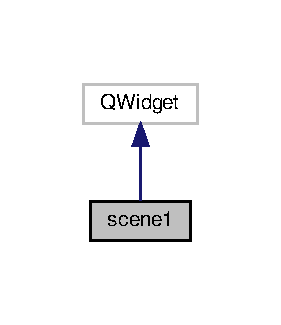
\includegraphics[width=135pt]{classscene1__inherit__graph}
\end{center}
\end{figure}


Collaboration diagram for scene1\+:
\nopagebreak
\begin{figure}[H]
\begin{center}
\leavevmode
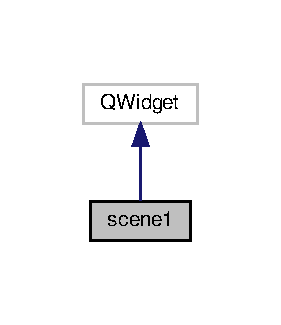
\includegraphics[width=135pt]{classscene1__coll__graph}
\end{center}
\end{figure}
\subsection*{Public Member Functions}
\begin{DoxyCompactItemize}
\item 
\hyperlink{classscene1_a55f27703d7a712de182d8b1d1a0c6885}{scene1} (Q\+Widget $\ast$parent=nullptr)
\begin{DoxyCompactList}\small\item\em \hyperlink{classscene1}{scene1} constructor \end{DoxyCompactList}\end{DoxyCompactItemize}


\subsection{Constructor \& Destructor Documentation}
\mbox{\Hypertarget{classscene1_a55f27703d7a712de182d8b1d1a0c6885}\label{classscene1_a55f27703d7a712de182d8b1d1a0c6885}} 
\index{scene1@{scene1}!scene1@{scene1}}
\index{scene1@{scene1}!scene1@{scene1}}
\subsubsection{\texorpdfstring{scene1()}{scene1()}}
{\footnotesize\ttfamily scene1\+::scene1 (\begin{DoxyParamCaption}\item[{Q\+Widget $\ast$}]{parent = {\ttfamily nullptr} }\end{DoxyParamCaption})\hspace{0.3cm}{\ttfamily [explicit]}}



\hyperlink{classscene1}{scene1} constructor 


\begin{DoxyParams}{Parameters}
{\em parent,a} & pointer to the parent widget \\
\hline
\end{DoxyParams}


The documentation for this class was generated from the following files\+:\begin{DoxyCompactItemize}
\item 
scene1.\+h\item 
scene1.\+cpp\end{DoxyCompactItemize}

\hypertarget{classsigninPage}{}\section{signin\+Page Class Reference}
\label{classsigninPage}\index{signin\+Page@{signin\+Page}}


Inheritance diagram for signin\+Page\+:
\nopagebreak
\begin{figure}[H]
\begin{center}
\leavevmode
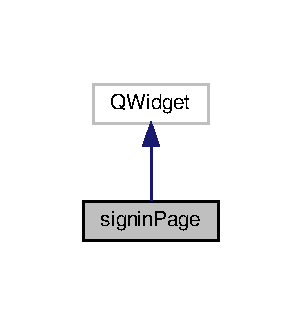
\includegraphics[width=145pt]{classsigninPage__inherit__graph}
\end{center}
\end{figure}


Collaboration diagram for signin\+Page\+:
\nopagebreak
\begin{figure}[H]
\begin{center}
\leavevmode
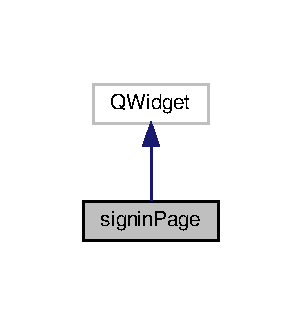
\includegraphics[width=145pt]{classsigninPage__coll__graph}
\end{center}
\end{figure}
\subsection*{Public Member Functions}
\begin{DoxyCompactItemize}
\item 
\hyperlink{classsigninPage_afb7dd0785bd1293840c5657b865ad841}{signin\+Page} (Q\+Widget $\ast$parent=nullptr)
\begin{DoxyCompactList}\small\item\em signing\+Page constructor \end{DoxyCompactList}\end{DoxyCompactItemize}


\subsection{Constructor \& Destructor Documentation}
\mbox{\Hypertarget{classsigninPage_afb7dd0785bd1293840c5657b865ad841}\label{classsigninPage_afb7dd0785bd1293840c5657b865ad841}} 
\index{signin\+Page@{signin\+Page}!signin\+Page@{signin\+Page}}
\index{signin\+Page@{signin\+Page}!signin\+Page@{signin\+Page}}
\subsubsection{\texorpdfstring{signin\+Page()}{signinPage()}}
{\footnotesize\ttfamily signin\+Page\+::signin\+Page (\begin{DoxyParamCaption}\item[{Q\+Widget $\ast$}]{parent = {\ttfamily nullptr} }\end{DoxyParamCaption})\hspace{0.3cm}{\ttfamily [explicit]}}



signing\+Page constructor 

\hyperlink{classsigninPage}{signin\+Page} constructor


\begin{DoxyParams}{Parameters}
{\em parent,a} & pointer to the parent widget \\
\hline
\end{DoxyParams}


The documentation for this class was generated from the following files\+:\begin{DoxyCompactItemize}
\item 
signinpage.\+h\item 
signinpage.\+cpp\end{DoxyCompactItemize}

\hypertarget{classsignup__scene}{}\section{signup\+\_\+scene Class Reference}
\label{classsignup__scene}\index{signup\+\_\+scene@{signup\+\_\+scene}}


Inheritance diagram for signup\+\_\+scene\+:
\nopagebreak
\begin{figure}[H]
\begin{center}
\leavevmode
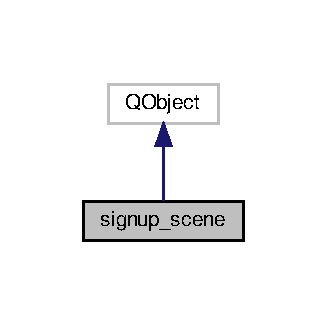
\includegraphics[width=157pt]{classsignup__scene__inherit__graph}
\end{center}
\end{figure}


Collaboration diagram for signup\+\_\+scene\+:
\nopagebreak
\begin{figure}[H]
\begin{center}
\leavevmode
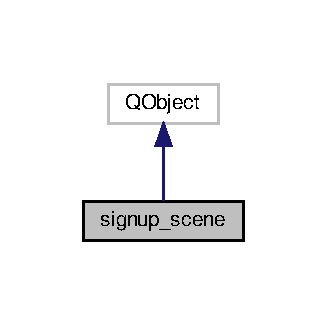
\includegraphics[width=157pt]{classsignup__scene__coll__graph}
\end{center}
\end{figure}
\subsection*{Public Member Functions}
\begin{DoxyCompactItemize}
\item 
\mbox{\Hypertarget{classsignup__scene_a451c908250948025fd79cfe2b9afb99c}\label{classsignup__scene_a451c908250948025fd79cfe2b9afb99c}} 
{\bfseries signup\+\_\+scene} (Q\+Object $\ast$parent=nullptr)
\end{DoxyCompactItemize}


The documentation for this class was generated from the following files\+:\begin{DoxyCompactItemize}
\item 
signup\+\_\+scene.\+h\item 
signup\+\_\+scene.\+cpp\end{DoxyCompactItemize}

\hypertarget{classsignupPage}{}\section{signup\+Page Class Reference}
\label{classsignupPage}\index{signup\+Page@{signup\+Page}}


Inheritance diagram for signup\+Page\+:
\nopagebreak
\begin{figure}[H]
\begin{center}
\leavevmode
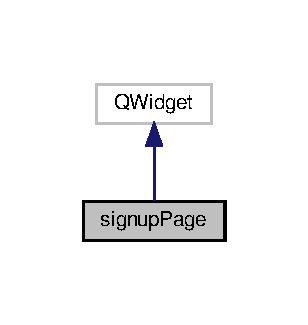
\includegraphics[width=148pt]{classsignupPage__inherit__graph}
\end{center}
\end{figure}


Collaboration diagram for signup\+Page\+:
\nopagebreak
\begin{figure}[H]
\begin{center}
\leavevmode
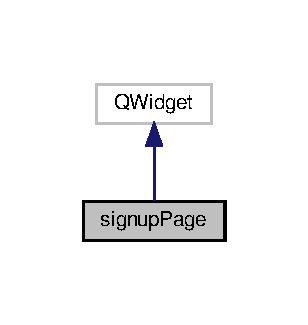
\includegraphics[width=148pt]{classsignupPage__coll__graph}
\end{center}
\end{figure}
\subsection*{Public Member Functions}
\begin{DoxyCompactItemize}
\item 
\hyperlink{classsignupPage_a98bc63ddaba1db86306d469223dc4c59}{signup\+Page} (Q\+Widget $\ast$parent=nullptr)
\begin{DoxyCompactList}\small\item\em \hyperlink{classsignupPage}{signup\+Page} constructor \end{DoxyCompactList}\end{DoxyCompactItemize}


\subsection{Constructor \& Destructor Documentation}
\mbox{\Hypertarget{classsignupPage_a98bc63ddaba1db86306d469223dc4c59}\label{classsignupPage_a98bc63ddaba1db86306d469223dc4c59}} 
\index{signup\+Page@{signup\+Page}!signup\+Page@{signup\+Page}}
\index{signup\+Page@{signup\+Page}!signup\+Page@{signup\+Page}}
\subsubsection{\texorpdfstring{signup\+Page()}{signupPage()}}
{\footnotesize\ttfamily signup\+Page\+::signup\+Page (\begin{DoxyParamCaption}\item[{Q\+Widget $\ast$}]{parent = {\ttfamily nullptr} }\end{DoxyParamCaption})\hspace{0.3cm}{\ttfamily [explicit]}}



\hyperlink{classsignupPage}{signup\+Page} constructor 


\begin{DoxyParams}{Parameters}
{\em parent,a} & pointer to the parent widget \\
\hline
\end{DoxyParams}


The documentation for this class was generated from the following files\+:\begin{DoxyCompactItemize}
\item 
signuppage.\+h\item 
signuppage.\+cpp\end{DoxyCompactItemize}

\hypertarget{classtimeUp}{}\section{time\+Up Class Reference}
\label{classtimeUp}\index{time\+Up@{time\+Up}}


Inheritance diagram for time\+Up\+:
\nopagebreak
\begin{figure}[H]
\begin{center}
\leavevmode
\includegraphics[width=135pt]{classtimeUp__inherit__graph}
\end{center}
\end{figure}


Collaboration diagram for time\+Up\+:
\nopagebreak
\begin{figure}[H]
\begin{center}
\leavevmode
\includegraphics[width=220pt]{classtimeUp__coll__graph}
\end{center}
\end{figure}
\subsection*{Public Member Functions}
\begin{DoxyCompactItemize}
\item 
\hyperlink{classtimeUp_a462717224a7754296209355928f97ab1}{time\+Up} (Q\+Widget $\ast$parent=nullptr, Q\+Json\+Object json=\{\}, int score\+Num=0, Q\+String game\+Id=\char`\"{}\char`\"{})
\begin{DoxyCompactList}\small\item\em \hyperlink{classtimeUp}{time\+Up} constructor \end{DoxyCompactList}\item 
\mbox{\Hypertarget{classtimeUp_afed188f978febdadc9c51ca2b510dedf}\label{classtimeUp_afed188f978febdadc9c51ca2b510dedf}} 
void \hyperlink{classtimeUp_afed188f978febdadc9c51ca2b510dedf}{init\+Bg} ()
\begin{DoxyCompactList}\small\item\em Initializes the bg of the widget. \end{DoxyCompactList}\item 
\mbox{\Hypertarget{classtimeUp_a050a9325077406b54bc32c332952327f}\label{classtimeUp_a050a9325077406b54bc32c332952327f}} 
void \hyperlink{classtimeUp_a050a9325077406b54bc32c332952327f}{check\+Score} ()
\begin{DoxyCompactList}\small\item\em checks if the score is a new highscore. If the condition is true, display congrats Q\+Label. \end{DoxyCompactList}\item 
int \hyperlink{classtimeUp_ae248b5d925d67ef28cb795147d260a93}{compute\+Bonus} ()
\begin{DoxyCompactList}\small\item\em compute\+Bonus, computes the bonus points a user gets in game 2 \end{DoxyCompactList}\end{DoxyCompactItemize}
\subsection*{Public Attributes}
\begin{DoxyCompactItemize}
\item 
\mbox{\Hypertarget{classtimeUp_ab10c6a95b213c06f95a289eb2a6c188e}\label{classtimeUp_ab10c6a95b213c06f95a289eb2a6c188e}} 
Q\+Json\+Object {\bfseries user\+Json}
\item 
\mbox{\Hypertarget{classtimeUp_a7c9045116d3a37e932441ae11e159ec6}\label{classtimeUp_a7c9045116d3a37e932441ae11e159ec6}} 
Q\+Label $\ast$ {\bfseries title}
\item 
\mbox{\Hypertarget{classtimeUp_ae5fd47a31b619e0a1f00234be0afbda5}\label{classtimeUp_ae5fd47a31b619e0a1f00234be0afbda5}} 
Q\+Label $\ast$ {\bfseries congrats}
\item 
\mbox{\Hypertarget{classtimeUp_a879a5bdb9943496d035c2b6a7ce97ad3}\label{classtimeUp_a879a5bdb9943496d035c2b6a7ce97ad3}} 
Q\+Label $\ast$ {\bfseries text}
\item 
\mbox{\Hypertarget{classtimeUp_adf2f4aa5469966f4f154c120d7a72227}\label{classtimeUp_adf2f4aa5469966f4f154c120d7a72227}} 
int {\bfseries score}
\item 
\mbox{\Hypertarget{classtimeUp_a5e31d3b089b22171726ed58df6c82041}\label{classtimeUp_a5e31d3b089b22171726ed58df6c82041}} 
Q\+String {\bfseries ID}
\item 
\mbox{\Hypertarget{classtimeUp_a61e7b1c71590020859f4a21b4b9af244}\label{classtimeUp_a61e7b1c71590020859f4a21b4b9af244}} 
Q\+Push\+Button $\ast$ {\bfseries exit\+Btn}
\item 
\mbox{\Hypertarget{classtimeUp_aca9594fa2b0e29fb397d2fb97d98b1e5}\label{classtimeUp_aca9594fa2b0e29fb397d2fb97d98b1e5}} 
Q\+V\+Box\+Layout $\ast$ {\bfseries v\+Layout}
\item 
\mbox{\Hypertarget{classtimeUp_a7569031bed14ca848099c05d2a5fd1a5}\label{classtimeUp_a7569031bed14ca848099c05d2a5fd1a5}} 
\hyperlink{classjsonhandler}{jsonhandler} $\ast$ {\bfseries jh} = new \hyperlink{classjsonhandler}{jsonhandler}()
\end{DoxyCompactItemize}


\subsection{Constructor \& Destructor Documentation}
\mbox{\Hypertarget{classtimeUp_a462717224a7754296209355928f97ab1}\label{classtimeUp_a462717224a7754296209355928f97ab1}} 
\index{time\+Up@{time\+Up}!time\+Up@{time\+Up}}
\index{time\+Up@{time\+Up}!time\+Up@{time\+Up}}
\subsubsection{\texorpdfstring{time\+Up()}{timeUp()}}
{\footnotesize\ttfamily time\+Up\+::time\+Up (\begin{DoxyParamCaption}\item[{Q\+Widget $\ast$}]{parent = {\ttfamily nullptr},  }\item[{Q\+Json\+Object}]{json = {\ttfamily \{\}},  }\item[{int}]{score\+Num = {\ttfamily 0},  }\item[{Q\+String}]{game\+Id = {\ttfamily \char`\"{}\char`\"{}} }\end{DoxyParamCaption})\hspace{0.3cm}{\ttfamily [explicit]}}



\hyperlink{classtimeUp}{time\+Up} constructor 


\begin{DoxyParams}{Parameters}
{\em parent,a} & pointer to a Q\+Widget parent \\
\hline
{\em json,a} & Q\+Json\+Object for a given user \\
\hline
{\em score\+Num,the} & player\textquotesingle{}s score. \\
\hline
{\em game\+Id,the} & game\textquotesingle{}s Id.\\
\hline
{\em parent,a} & pointer to a Q\+Widget parent \\
\hline
{\em json,a} & Q\+Json\+Object for a given user \\
\hline
{\em score\+Num,the} & player\textquotesingle{}s score. \\
\hline
{\em game\+Id,Q\+String} & that specifies which game is being played. \\
\hline
\end{DoxyParams}


\subsection{Member Function Documentation}
\mbox{\Hypertarget{classtimeUp_ae248b5d925d67ef28cb795147d260a93}\label{classtimeUp_ae248b5d925d67ef28cb795147d260a93}} 
\index{time\+Up@{time\+Up}!compute\+Bonus@{compute\+Bonus}}
\index{compute\+Bonus@{compute\+Bonus}!time\+Up@{time\+Up}}
\subsubsection{\texorpdfstring{compute\+Bonus()}{computeBonus()}}
{\footnotesize\ttfamily int time\+Up\+::compute\+Bonus (\begin{DoxyParamCaption}{ }\end{DoxyParamCaption})}



compute\+Bonus, computes the bonus points a user gets in game 2 

\hyperlink{classtimeUp_ae248b5d925d67ef28cb795147d260a93}{time\+Up\+::compute\+Bonus}, computes the bonus points earned in game 2

\begin{DoxyReturn}{Returns}
an integer, the bonus points. If bonus points is a negative number, it returns 0.

int, the bonus points 
\end{DoxyReturn}


The documentation for this class was generated from the following files\+:\begin{DoxyCompactItemize}
\item 
timeup.\+h\item 
timeup.\+cpp\end{DoxyCompactItemize}

\chapter{File Documentation}
\hypertarget{account_8cpp}{}\section{account.\+cpp File Reference}
\label{account_8cpp}\index{account.\+cpp@{account.\+cpp}}


the account widget  


{\ttfamily \#include \char`\"{}account.\+h\char`\"{}}\newline
Include dependency graph for account.\+cpp\+:
\nopagebreak
\begin{figure}[H]
\begin{center}
\leavevmode
\includegraphics[width=350pt]{account_8cpp__incl}
\end{center}
\end{figure}


\subsection{Detailed Description}
the account widget 

This widget includes two main widgets\+: the \hyperlink{classaccount__sidebar}{account\+\_\+sidebar} and the \hyperlink{classaccount__dashboard}{account\+\_\+dashboard} 
\hypertarget{account_8h}{}\section{account.\+h File Reference}
\label{account_8h}\index{account.\+h@{account.\+h}}


the account widget  


{\ttfamily \#include $<$Q\+Object$>$}\newline
{\ttfamily \#include $<$Q\+Widget$>$}\newline
{\ttfamily \#include $<$Qt\+Widgets$>$}\newline
{\ttfamily \#include \char`\"{}account\+\_\+sidebar.\+h\char`\"{}}\newline
{\ttfamily \#include \char`\"{}account\+\_\+dashboard.\+h\char`\"{}}\newline
Include dependency graph for account.\+h\+:
\nopagebreak
\begin{figure}[H]
\begin{center}
\leavevmode
\includegraphics[width=350pt]{account_8h__incl}
\end{center}
\end{figure}
This graph shows which files directly or indirectly include this file\+:
\nopagebreak
\begin{figure}[H]
\begin{center}
\leavevmode
\includegraphics[width=350pt]{account_8h__dep__incl}
\end{center}
\end{figure}
\subsection*{Classes}
\begin{DoxyCompactItemize}
\item 
class \hyperlink{classaccount}{account}
\end{DoxyCompactItemize}


\subsection{Detailed Description}
the account widget 

This widget includes two main widgets\+: the \hyperlink{classaccount__sidebar}{account\+\_\+sidebar} and the \hyperlink{classaccount__dashboard}{account\+\_\+dashboard} 
\hypertarget{account__dashboard_8cpp}{}\section{account\+\_\+dashboard.\+cpp File Reference}
\label{account__dashboard_8cpp}\index{account\+\_\+dashboard.\+cpp@{account\+\_\+dashboard.\+cpp}}


the \hyperlink{classaccount__dashboard}{account\+\_\+dashboard} widget  


{\ttfamily \#include \char`\"{}account\+\_\+dashboard.\+h\char`\"{}}\newline
Include dependency graph for account\+\_\+dashboard.\+cpp\+:
\nopagebreak
\begin{figure}[H]
\begin{center}
\leavevmode
\includegraphics[width=350pt]{account__dashboard_8cpp__incl}
\end{center}
\end{figure}


\subsection{Detailed Description}
the \hyperlink{classaccount__dashboard}{account\+\_\+dashboard} widget 

This widget displays a game stats. The stats include user highscore, global highscore, user rank, and a performance plot based on the user scores. 
\hypertarget{account__dashboard_8h}{}\section{account\+\_\+dashboard.\+h File Reference}
\label{account__dashboard_8h}\index{account\+\_\+dashboard.\+h@{account\+\_\+dashboard.\+h}}


the \hyperlink{classaccount__dashboard}{account\+\_\+dashboard} widget  


{\ttfamily \#include $<$Q\+Widget$>$}\newline
{\ttfamily \#include $<$Qt\+Widgets$>$}\newline
{\ttfamily \#include $<$Qt\+Charts/\+Q\+Chart$>$}\newline
{\ttfamily \#include $<$Qt\+Charts/\+Q\+Line\+Series$>$}\newline
{\ttfamily \#include $<$Qt\+Charts/\+Q\+Chart\+View$>$}\newline
{\ttfamily \#include \char`\"{}jsonhandler.\+h\char`\"{}}\newline
Include dependency graph for account\+\_\+dashboard.\+h\+:
\nopagebreak
\begin{figure}[H]
\begin{center}
\leavevmode
\includegraphics[width=350pt]{account__dashboard_8h__incl}
\end{center}
\end{figure}
This graph shows which files directly or indirectly include this file\+:
\nopagebreak
\begin{figure}[H]
\begin{center}
\leavevmode
\includegraphics[width=350pt]{account__dashboard_8h__dep__incl}
\end{center}
\end{figure}
\subsection*{Classes}
\begin{DoxyCompactItemize}
\item 
class \hyperlink{classaccount__dashboard}{account\+\_\+dashboard}
\end{DoxyCompactItemize}


\subsection{Detailed Description}
the \hyperlink{classaccount__dashboard}{account\+\_\+dashboard} widget 

This widget displays a game stats. The stats include user highscore, global highscore, user rank, and a performance plot based on the user scores. 
\hypertarget{account__sidebar_8cpp}{}\section{account\+\_\+sidebar.\+cpp File Reference}
\label{account__sidebar_8cpp}\index{account\+\_\+sidebar.\+cpp@{account\+\_\+sidebar.\+cpp}}


This widget constructs the sidebar of the account widget.  


{\ttfamily \#include \char`\"{}account\+\_\+sidebar.\+h\char`\"{}}\newline
{\ttfamily \#include \char`\"{}account.\+h\char`\"{}}\newline
{\ttfamily \#include \char`\"{}scene1.\+h\char`\"{}}\newline
{\ttfamily \#include \char`\"{}g1\+\_\+startmenu.\+h\char`\"{}}\newline
{\ttfamily \#include \char`\"{}g2\+\_\+startmenu.\+h\char`\"{}}\newline
{\ttfamily \#include \char`\"{}centering.\+h\char`\"{}}\newline
Include dependency graph for account\+\_\+sidebar.\+cpp\+:
\nopagebreak
\begin{figure}[H]
\begin{center}
\leavevmode
\includegraphics[width=350pt]{account__sidebar_8cpp__incl}
\end{center}
\end{figure}


\subsection{Detailed Description}
This widget constructs the sidebar of the account widget. 

The sidebar includes information about the user. It also includes navigation buttons. 
\hypertarget{account__sidebar_8h}{}\section{account\+\_\+sidebar.\+h File Reference}
\label{account__sidebar_8h}\index{account\+\_\+sidebar.\+h@{account\+\_\+sidebar.\+h}}


This widget constructs the sidebar of the account widget.  


{\ttfamily \#include $<$Q\+Object$>$}\newline
{\ttfamily \#include $<$Q\+Widget$>$}\newline
{\ttfamily \#include $<$Qt\+Widgets$>$}\newline
{\ttfamily \#include $<$Q\+Json\+Object$>$}\newline
Include dependency graph for account\+\_\+sidebar.\+h\+:
\nopagebreak
\begin{figure}[H]
\begin{center}
\leavevmode
\includegraphics[width=350pt]{account__sidebar_8h__incl}
\end{center}
\end{figure}
This graph shows which files directly or indirectly include this file\+:
\nopagebreak
\begin{figure}[H]
\begin{center}
\leavevmode
\includegraphics[width=350pt]{account__sidebar_8h__dep__incl}
\end{center}
\end{figure}
\subsection*{Classes}
\begin{DoxyCompactItemize}
\item 
class \hyperlink{classaccount__sidebar}{account\+\_\+sidebar}
\end{DoxyCompactItemize}


\subsection{Detailed Description}
This widget constructs the sidebar of the account widget. 

The sidebar includes information about the user. It also includes navigation buttons. 
\hypertarget{butb_8cpp}{}\section{butb.\+cpp File Reference}
\label{butb_8cpp}\index{butb.\+cpp@{butb.\+cpp}}


the blue disk in game 2  


{\ttfamily \#include \char`\"{}butb.\+h\char`\"{}}\newline
{\ttfamily \#include $<$Q\+Debug$>$}\newline
Include dependency graph for butb.\+cpp\+:
\nopagebreak
\begin{figure}[H]
\begin{center}
\leavevmode
\includegraphics[width=350pt]{butb_8cpp__incl}
\end{center}
\end{figure}


\subsection{Detailed Description}
the blue disk in game 2 


\hypertarget{butb_8h}{}\section{butb.\+h File Reference}
\label{butb_8h}\index{butb.\+h@{butb.\+h}}


the blue disk in game 2  


{\ttfamily \#include $<$Q\+Object$>$}\newline
{\ttfamily \#include $<$Q\+Timer$>$}\newline
{\ttfamily \#include $<$Q\+Pixmap$>$}\newline
{\ttfamily \#include $<$Q\+Graphics\+Pixmap\+Item$>$}\newline
{\ttfamily \#include $<$Q\+Graphics\+Scene$>$}\newline
{\ttfamily \#include $<$Q\+Label$>$}\newline
{\ttfamily \#include $<$Q\+Graphics\+View$>$}\newline
{\ttfamily \#include $<$Q\+Graphics\+Item$>$}\newline
{\ttfamily \#include \char`\"{}butblack.\+h\char`\"{}}\newline
Include dependency graph for butb.\+h\+:
\nopagebreak
\begin{figure}[H]
\begin{center}
\leavevmode
\includegraphics[width=350pt]{butb_8h__incl}
\end{center}
\end{figure}
This graph shows which files directly or indirectly include this file\+:
\nopagebreak
\begin{figure}[H]
\begin{center}
\leavevmode
\includegraphics[width=350pt]{butb_8h__dep__incl}
\end{center}
\end{figure}
\subsection*{Classes}
\begin{DoxyCompactItemize}
\item 
class \hyperlink{classbutb}{butb}
\end{DoxyCompactItemize}


\subsection{Detailed Description}
the blue disk in game 2 


\hypertarget{butblack_8cpp}{}\section{butblack.\+cpp File Reference}
\label{butblack_8cpp}\index{butblack.\+cpp@{butblack.\+cpp}}


the grey disk in game 2  


{\ttfamily \#include \char`\"{}butblack.\+h\char`\"{}}\newline
{\ttfamily \#include $<$Q\+Debug$>$}\newline
Include dependency graph for butblack.\+cpp\+:
\nopagebreak
\begin{figure}[H]
\begin{center}
\leavevmode
\includegraphics[width=350pt]{butblack_8cpp__incl}
\end{center}
\end{figure}


\subsection{Detailed Description}
the grey disk in game 2 


\hypertarget{butblack_8h}{}\section{butblack.\+h File Reference}
\label{butblack_8h}\index{butblack.\+h@{butblack.\+h}}


the grey disk in game 2  


{\ttfamily \#include $<$Q\+Object$>$}\newline
{\ttfamily \#include $<$Q\+Timer$>$}\newline
{\ttfamily \#include $<$Q\+Pixmap$>$}\newline
{\ttfamily \#include $<$Q\+Graphics\+Pixmap\+Item$>$}\newline
{\ttfamily \#include $<$Q\+Graphics\+Scene$>$}\newline
{\ttfamily \#include $<$Q\+Label$>$}\newline
{\ttfamily \#include $<$Q\+Graphics\+View$>$}\newline
{\ttfamily \#include $<$Q\+Graphics\+Item$>$}\newline
Include dependency graph for butblack.\+h\+:
\nopagebreak
\begin{figure}[H]
\begin{center}
\leavevmode
\includegraphics[width=350pt]{butblack_8h__incl}
\end{center}
\end{figure}
This graph shows which files directly or indirectly include this file\+:
\nopagebreak
\begin{figure}[H]
\begin{center}
\leavevmode
\includegraphics[width=350pt]{butblack_8h__dep__incl}
\end{center}
\end{figure}
\subsection*{Classes}
\begin{DoxyCompactItemize}
\item 
class \hyperlink{classbutblack}{butblack}
\end{DoxyCompactItemize}


\subsection{Detailed Description}
the grey disk in game 2 


\hypertarget{butg_8cpp}{}\section{butg.\+cpp File Reference}
\label{butg_8cpp}\index{butg.\+cpp@{butg.\+cpp}}


the green disk in game 2  


{\ttfamily \#include \char`\"{}butg.\+h\char`\"{}}\newline
{\ttfamily \#include $<$Q\+Debug$>$}\newline
Include dependency graph for butg.\+cpp\+:
\nopagebreak
\begin{figure}[H]
\begin{center}
\leavevmode
\includegraphics[width=350pt]{butg_8cpp__incl}
\end{center}
\end{figure}


\subsection{Detailed Description}
the green disk in game 2 


\hypertarget{butg_8h}{}\section{butg.\+h File Reference}
\label{butg_8h}\index{butg.\+h@{butg.\+h}}


the green disk in game 2  


{\ttfamily \#include $<$Q\+Object$>$}\newline
{\ttfamily \#include $<$Q\+Timer$>$}\newline
{\ttfamily \#include $<$Q\+Pixmap$>$}\newline
{\ttfamily \#include $<$Q\+Graphics\+Pixmap\+Item$>$}\newline
{\ttfamily \#include $<$Q\+Graphics\+Scene$>$}\newline
{\ttfamily \#include $<$Q\+Label$>$}\newline
{\ttfamily \#include $<$Q\+Graphics\+View$>$}\newline
{\ttfamily \#include $<$Q\+Graphics\+Item$>$}\newline
{\ttfamily \#include \char`\"{}butblack.\+h\char`\"{}}\newline
Include dependency graph for butg.\+h\+:
\nopagebreak
\begin{figure}[H]
\begin{center}
\leavevmode
\includegraphics[width=350pt]{butg_8h__incl}
\end{center}
\end{figure}
This graph shows which files directly or indirectly include this file\+:
\nopagebreak
\begin{figure}[H]
\begin{center}
\leavevmode
\includegraphics[width=350pt]{butg_8h__dep__incl}
\end{center}
\end{figure}
\subsection*{Classes}
\begin{DoxyCompactItemize}
\item 
class \hyperlink{classbutg}{butg}
\end{DoxyCompactItemize}


\subsection{Detailed Description}
the green disk in game 2 


\hypertarget{butp_8cpp}{}\section{butp.\+cpp File Reference}
\label{butp_8cpp}\index{butp.\+cpp@{butp.\+cpp}}


the purple disk in game 2  


{\ttfamily \#include \char`\"{}butp.\+h\char`\"{}}\newline
{\ttfamily \#include $<$Q\+Debug$>$}\newline
Include dependency graph for butp.\+cpp\+:
\nopagebreak
\begin{figure}[H]
\begin{center}
\leavevmode
\includegraphics[width=350pt]{butp_8cpp__incl}
\end{center}
\end{figure}


\subsection{Detailed Description}
the purple disk in game 2 


\hypertarget{butp_8h}{}\section{butp.\+h File Reference}
\label{butp_8h}\index{butp.\+h@{butp.\+h}}


the purple disk in game 2  


{\ttfamily \#include $<$Q\+Object$>$}\newline
{\ttfamily \#include $<$Q\+Timer$>$}\newline
{\ttfamily \#include $<$Q\+Pixmap$>$}\newline
{\ttfamily \#include $<$Q\+Graphics\+Pixmap\+Item$>$}\newline
{\ttfamily \#include $<$Q\+Graphics\+Scene$>$}\newline
{\ttfamily \#include $<$Q\+Label$>$}\newline
{\ttfamily \#include $<$Q\+Graphics\+View$>$}\newline
{\ttfamily \#include $<$Q\+Graphics\+Item$>$}\newline
{\ttfamily \#include \char`\"{}butblack.\+h\char`\"{}}\newline
Include dependency graph for butp.\+h\+:
\nopagebreak
\begin{figure}[H]
\begin{center}
\leavevmode
\includegraphics[width=350pt]{butp_8h__incl}
\end{center}
\end{figure}
This graph shows which files directly or indirectly include this file\+:
\nopagebreak
\begin{figure}[H]
\begin{center}
\leavevmode
\includegraphics[width=350pt]{butp_8h__dep__incl}
\end{center}
\end{figure}
\subsection*{Classes}
\begin{DoxyCompactItemize}
\item 
class \hyperlink{classbutp}{butp}
\end{DoxyCompactItemize}


\subsection{Detailed Description}
the purple disk in game 2 


\hypertarget{g1__info_8cpp}{}\section{g1\+\_\+info.\+cpp File Reference}
\label{g1__info_8cpp}\index{g1\+\_\+info.\+cpp@{g1\+\_\+info.\+cpp}}


this class is a widget that informs the player on how to play Battleships.  


{\ttfamily \#include \char`\"{}g1\+\_\+info.\+h\char`\"{}}\newline
Include dependency graph for g1\+\_\+info.\+cpp\+:
\nopagebreak
\begin{figure}[H]
\begin{center}
\leavevmode
\includegraphics[width=350pt]{g1__info_8cpp__incl}
\end{center}
\end{figure}


\subsection{Detailed Description}
this class is a widget that informs the player on how to play Battleships. 


\hypertarget{g1__info_8h}{}\section{g1\+\_\+info.\+h File Reference}
\label{g1__info_8h}\index{g1\+\_\+info.\+h@{g1\+\_\+info.\+h}}


this class is a widget that informs the player on how to play Battleships.  


{\ttfamily \#include $<$Q\+Main\+Window$>$}\newline
{\ttfamily \#include $<$Q\+Object$>$}\newline
{\ttfamily \#include $<$Q\+Widget$>$}\newline
{\ttfamily \#include $<$Qt\+Widgets$>$}\newline
{\ttfamily \#include \char`\"{}jsonhandler.\+h\char`\"{}}\newline
{\ttfamily \#include \char`\"{}g1\+\_\+setup.\+h\char`\"{}}\newline
Include dependency graph for g1\+\_\+info.\+h\+:
\nopagebreak
\begin{figure}[H]
\begin{center}
\leavevmode
\includegraphics[width=350pt]{g1__info_8h__incl}
\end{center}
\end{figure}
This graph shows which files directly or indirectly include this file\+:
\nopagebreak
\begin{figure}[H]
\begin{center}
\leavevmode
\includegraphics[width=350pt]{g1__info_8h__dep__incl}
\end{center}
\end{figure}
\subsection*{Classes}
\begin{DoxyCompactItemize}
\item 
class \hyperlink{classg1__info}{g1\+\_\+info}
\end{DoxyCompactItemize}


\subsection{Detailed Description}
this class is a widget that informs the player on how to play Battleships. 


\hypertarget{g1__settings_8h}{}\section{g1\+\_\+settings.\+h File Reference}
\label{g1__settings_8h}\index{g1\+\_\+settings.\+h@{g1\+\_\+settings.\+h}}


A widget that displays a game settings window.  


{\ttfamily \#include $<$Q\+Object$>$}\newline
{\ttfamily \#include $<$Q\+Widget$>$}\newline
{\ttfamily \#include $<$Qt\+Widgets$>$}\newline
{\ttfamily \#include \char`\"{}jsonhandler.\+h\char`\"{}}\newline
Include dependency graph for g1\+\_\+settings.\+h\+:
\nopagebreak
\begin{figure}[H]
\begin{center}
\leavevmode
\includegraphics[width=350pt]{g1__settings_8h__incl}
\end{center}
\end{figure}
This graph shows which files directly or indirectly include this file\+:
\nopagebreak
\begin{figure}[H]
\begin{center}
\leavevmode
\includegraphics[width=175pt]{g1__settings_8h__dep__incl}
\end{center}
\end{figure}
\subsection*{Classes}
\begin{DoxyCompactItemize}
\item 
class \hyperlink{classg1__settings}{g1\+\_\+settings}
\end{DoxyCompactItemize}


\subsection{Detailed Description}
A widget that displays a game settings window. 


\hypertarget{g1__startmenu_8cpp}{}\section{g1\+\_\+startmenu.\+cpp File Reference}
\label{g1__startmenu_8cpp}\index{g1\+\_\+startmenu.\+cpp@{g1\+\_\+startmenu.\+cpp}}


the start menu of Battleships  


{\ttfamily \#include \char`\"{}g1\+\_\+settings.\+h\char`\"{}}\newline
{\ttfamily \#include \char`\"{}g1\+\_\+setup.\+h\char`\"{}}\newline
{\ttfamily \#include \char`\"{}account.\+h\char`\"{}}\newline
{\ttfamily \#include \char`\"{}centering.\+h\char`\"{}}\newline
{\ttfamily \#include \char`\"{}g1\+\_\+startmenu.\+h\char`\"{}}\newline
Include dependency graph for g1\+\_\+startmenu.\+cpp\+:
\nopagebreak
\begin{figure}[H]
\begin{center}
\leavevmode
\includegraphics[width=350pt]{g1__startmenu_8cpp__incl}
\end{center}
\end{figure}


\subsection{Detailed Description}
the start menu of Battleships 


\hypertarget{g1__startmenu_8h}{}\section{g1\+\_\+startmenu.\+h File Reference}
\label{g1__startmenu_8h}\index{g1\+\_\+startmenu.\+h@{g1\+\_\+startmenu.\+h}}


the start menu of Battleships  


{\ttfamily \#include $<$Q\+Widget$>$}\newline
{\ttfamily \#include $<$Q\+Push\+Button$>$}\newline
{\ttfamily \#include $<$Q\+V\+Box\+Layout$>$}\newline
{\ttfamily \#include $<$Q\+Label$>$}\newline
{\ttfamily \#include $<$Q\+Json\+Object$>$}\newline
{\ttfamily \#include \char`\"{}jsonhandler.\+h\char`\"{}}\newline
{\ttfamily \#include \char`\"{}account.\+h\char`\"{}}\newline
{\ttfamily \#include \char`\"{}g1\+\_\+info.\+h\char`\"{}}\newline
Include dependency graph for g1\+\_\+startmenu.\+h\+:
\nopagebreak
\begin{figure}[H]
\begin{center}
\leavevmode
\includegraphics[width=350pt]{g1__startmenu_8h__incl}
\end{center}
\end{figure}
This graph shows which files directly or indirectly include this file\+:
\nopagebreak
\begin{figure}[H]
\begin{center}
\leavevmode
\includegraphics[width=350pt]{g1__startmenu_8h__dep__incl}
\end{center}
\end{figure}
\subsection*{Classes}
\begin{DoxyCompactItemize}
\item 
class \hyperlink{classg1__startmenu}{g1\+\_\+startmenu}
\end{DoxyCompactItemize}


\subsection{Detailed Description}
the start menu of Battleships 


\hypertarget{g2__settings_8cpp}{}\section{g2\+\_\+settings.\+cpp File Reference}
\label{g2__settings_8cpp}\index{g2\+\_\+settings.\+cpp@{g2\+\_\+settings.\+cpp}}


This class creates the settings Q\+Widget for Shooting discs. In the settings, the user can change the game difficulty and background image. Changing the difficulty changes the target score and lives. Changing the background updates the image of the gameplay O\+N\+LY. (unlike Battleships, the start menu and settings do not change backgrounds).  


{\ttfamily \#include \char`\"{}g2\+\_\+settings.\+h\char`\"{}}\newline
{\ttfamily \#include \char`\"{}g2\+\_\+setup.\+h\char`\"{}}\newline
{\ttfamily \#include \char`\"{}g2\+\_\+startmenu.\+h\char`\"{}}\newline
{\ttfamily \#include \char`\"{}centering.\+h\char`\"{}}\newline
Include dependency graph for g2\+\_\+settings.\+cpp\+:
\nopagebreak
\begin{figure}[H]
\begin{center}
\leavevmode
\includegraphics[width=350pt]{g2__settings_8cpp__incl}
\end{center}
\end{figure}


\subsection{Detailed Description}
This class creates the settings Q\+Widget for Shooting discs. In the settings, the user can change the game difficulty and background image. Changing the difficulty changes the target score and lives. Changing the background updates the image of the gameplay O\+N\+LY. (unlike Battleships, the start menu and settings do not change backgrounds). 


\hypertarget{g2__settings_8h}{}\section{g2\+\_\+settings.\+h File Reference}
\label{g2__settings_8h}\index{g2\+\_\+settings.\+h@{g2\+\_\+settings.\+h}}


This class creates the settings Q\+Widget for Shooting discs. In the settings, the user can change the game difficulty and background image. Changing the difficulty changes the target score and lives. Changing the background updates the image of the gameplay O\+N\+LY. (unlike Battleships, the start menu and settings do not change backgrounds).  


{\ttfamily \#include $<$Q\+Widget$>$}\newline
{\ttfamily \#include $<$Qt\+Widgets$>$}\newline
{\ttfamily \#include \char`\"{}jsonhandler.\+h\char`\"{}}\newline
Include dependency graph for g2\+\_\+settings.\+h\+:
\nopagebreak
\begin{figure}[H]
\begin{center}
\leavevmode
\includegraphics[width=350pt]{g2__settings_8h__incl}
\end{center}
\end{figure}
This graph shows which files directly or indirectly include this file\+:
\nopagebreak
\begin{figure}[H]
\begin{center}
\leavevmode
\includegraphics[width=350pt]{g2__settings_8h__dep__incl}
\end{center}
\end{figure}
\subsection*{Classes}
\begin{DoxyCompactItemize}
\item 
class \hyperlink{classg2__settings}{g2\+\_\+settings}
\end{DoxyCompactItemize}


\subsection{Detailed Description}
This class creates the settings Q\+Widget for Shooting discs. In the settings, the user can change the game difficulty and background image. Changing the difficulty changes the target score and lives. Changing the background updates the image of the gameplay O\+N\+LY. (unlike Battleships, the start menu and settings do not change backgrounds). 


\hypertarget{g2__startmenu_8h}{}\section{g2\+\_\+startmenu.\+h File Reference}
\label{g2__startmenu_8h}\index{g2\+\_\+startmenu.\+h@{g2\+\_\+startmenu.\+h}}


the start menu of Shooting Disks  


{\ttfamily \#include $<$Q\+Object$>$}\newline
{\ttfamily \#include $<$Q\+Widget$>$}\newline
{\ttfamily \#include $<$Qt\+Widgets$>$}\newline
{\ttfamily \#include \char`\"{}jsonhandler.\+h\char`\"{}}\newline
{\ttfamily \#include \char`\"{}account.\+h\char`\"{}}\newline
{\ttfamily \#include \char`\"{}g2\+\_\+settings.\+h\char`\"{}}\newline
{\ttfamily \#include \char`\"{}g2\+\_\+setup.\+h\char`\"{}}\newline
{\ttfamily \#include \char`\"{}centering.\+h\char`\"{}}\newline
Include dependency graph for g2\+\_\+startmenu.\+h\+:
\nopagebreak
\begin{figure}[H]
\begin{center}
\leavevmode
\includegraphics[width=350pt]{g2__startmenu_8h__incl}
\end{center}
\end{figure}
This graph shows which files directly or indirectly include this file\+:
\nopagebreak
\begin{figure}[H]
\begin{center}
\leavevmode
\includegraphics[width=350pt]{g2__startmenu_8h__dep__incl}
\end{center}
\end{figure}
\subsection*{Classes}
\begin{DoxyCompactItemize}
\item 
class \hyperlink{classg2__startmenu}{g2\+\_\+startmenu}
\end{DoxyCompactItemize}


\subsection{Detailed Description}
the start menu of Shooting Disks 


\hypertarget{jsonhandler_8cpp}{}\section{jsonhandler.\+cpp File Reference}
\label{jsonhandler_8cpp}\index{jsonhandler.\+cpp@{jsonhandler.\+cpp}}


A class that allows us to perform queries on the json file or a json object.  


{\ttfamily \#include \char`\"{}jsonhandler.\+h\char`\"{}}\newline
{\ttfamily \#include $<$Q\+Debug$>$}\newline
Include dependency graph for jsonhandler.\+cpp\+:
\nopagebreak
\begin{figure}[H]
\begin{center}
\leavevmode
\includegraphics[width=350pt]{jsonhandler_8cpp__incl}
\end{center}
\end{figure}


\subsection{Detailed Description}
A class that allows us to perform queries on the json file or a json object. 


\hypertarget{jsonhandler_8h}{}\section{jsonhandler.\+h File Reference}
\label{jsonhandler_8h}\index{jsonhandler.\+h@{jsonhandler.\+h}}


A class that allows us to perform queries on the json file or a json object.  


{\ttfamily \#include $<$Q\+Object$>$}\newline
{\ttfamily \#include $<$Q\+File$>$}\newline
{\ttfamily \#include $<$Q\+Json\+Array$>$}\newline
{\ttfamily \#include $<$Q\+Json\+Object$>$}\newline
{\ttfamily \#include $<$Q\+Json\+Document$>$}\newline
{\ttfamily \#include $<$Q\+Message\+Box$>$}\newline
{\ttfamily \#include $<$Q\+List$>$}\newline
{\ttfamily \#include $<$bits/stdc++.\+h$>$}\newline
{\ttfamily \#include $<$Qt\+Algorithms$>$}\newline
Include dependency graph for jsonhandler.\+h\+:
\nopagebreak
\begin{figure}[H]
\begin{center}
\leavevmode
\includegraphics[width=350pt]{jsonhandler_8h__incl}
\end{center}
\end{figure}
This graph shows which files directly or indirectly include this file\+:
\nopagebreak
\begin{figure}[H]
\begin{center}
\leavevmode
\includegraphics[width=350pt]{jsonhandler_8h__dep__incl}
\end{center}
\end{figure}
\subsection*{Classes}
\begin{DoxyCompactItemize}
\item 
class \hyperlink{classjsonhandler}{jsonhandler}
\end{DoxyCompactItemize}


\subsection{Detailed Description}
A class that allows us to perform queries on the json file or a json object. 


\hypertarget{quests_8cpp}{}\section{quests.\+cpp File Reference}
\label{quests_8cpp}\index{quests.\+cpp@{quests.\+cpp}}


A class that displays a Q\+Dialog of a question in Battleships game This class contains queries to the questions.\+json file.  


{\ttfamily \#include \char`\"{}quests.\+h\char`\"{}}\newline
{\ttfamily \#include $<$Q\+Debug$>$}\newline
{\ttfamily \#include $<$Q\+Object$>$}\newline
Include dependency graph for quests.\+cpp\+:
\nopagebreak
\begin{figure}[H]
\begin{center}
\leavevmode
\includegraphics[width=350pt]{quests_8cpp__incl}
\end{center}
\end{figure}


\subsection{Detailed Description}
A class that displays a Q\+Dialog of a question in Battleships game This class contains queries to the questions.\+json file. 


\hypertarget{quests_8h}{}\section{quests.\+h File Reference}
\label{quests_8h}\index{quests.\+h@{quests.\+h}}


A class that displays a Q\+Dialog of a question in Battleships game This class contains queries to the questions.\+json file.  


{\ttfamily \#include $<$jsonhandler.\+h$>$}\newline
{\ttfamily \#include $<$Q\+Object$>$}\newline
{\ttfamily \#include $<$Q\+Widget$>$}\newline
{\ttfamily \#include $<$Q\+Label$>$}\newline
{\ttfamily \#include $<$Q\+Push\+Button$>$}\newline
{\ttfamily \#include $<$Q\+V\+Box\+Layout$>$}\newline
{\ttfamily \#include $<$Q\+Group\+Box$>$}\newline
{\ttfamily \#include $<$Q\+Message\+Box$>$}\newline
{\ttfamily \#include $<$Q\+Json\+Array$>$}\newline
{\ttfamily \#include $<$Q\+Json\+Object$>$}\newline
{\ttfamily \#include \char`\"{}g1\+\_\+setup.\+h\char`\"{}}\newline
Include dependency graph for quests.\+h\+:
\nopagebreak
\begin{figure}[H]
\begin{center}
\leavevmode
\includegraphics[width=350pt]{quests_8h__incl}
\end{center}
\end{figure}
This graph shows which files directly or indirectly include this file\+:
\nopagebreak
\begin{figure}[H]
\begin{center}
\leavevmode
\includegraphics[width=350pt]{quests_8h__dep__incl}
\end{center}
\end{figure}
\subsection*{Classes}
\begin{DoxyCompactItemize}
\item 
class \hyperlink{classquests}{quests}
\end{DoxyCompactItemize}


\subsection{Detailed Description}
A class that displays a Q\+Dialog of a question in Battleships game This class contains queries to the questions.\+json file. 


%--- End generated contents ---

% Index
\backmatter
\newpage
\phantomsection
\clearemptydoublepage
\addcontentsline{toc}{chapter}{Index}
\printindex

\end{document}
